\section{Analysis Results}
\subsection{Final Expression and Validation}
\begin{frame}{Important Parameters Revealed by Fourier Analysis}
\vspace{-1em}
\begin{itemize}
    \item Definition and Range
    \begin{table} [!hbt]
    \centering
     \small
    \begin{tabular}{c| P{2cm}|P{2cm}|P{2cm}|P{2cm}} 
        \toprule
         \textbf{Symbol}&c & $\gamma$ & $r$ & $\Sigma_tX$\\ 
        \midrule
       \textbf{Definition}&Scattering Ratio & Feedback intensity & Wielandt shift ratio & Problem Size (mfp)\\
        \midrule
        \textbf{Range}&$<0.96$ & $0-0.00121$ & $0.66-0.99$& $<500$\\ 
        \toprule
    \end{tabular}
    \end{table}
    \item Mathematical Expression:
\end{itemize}
% \begin{multicols}{4}
%   \begin{equation}
%     c=\frac{\Sigma_{s,0}}{\Sigma_{t,0}}
%   \end{equation}\break
%   \begin{equation}
%     \gamma_0= \left(\frac{\Sigma_{a,1}}{\Sigma_{a,0}} - \frac{ \Sigma_{f,1}}{\Sigma_{f,0}}\right) \Phi_0
%   \end{equation}\break\\
%   \begin{equation}
%   \frac{d\lambda}{d\phi}\frac{\nu\Sigma_{f,0}}{{\Sigma_{t,0}}}\label{eq:gamma_def}
%   \end{equation}
%   \begin{equation}
% r=\frac{\lambda_s}{\lambda}
%   \end{equation}
% \end{multicols}
\vspace{-1em}
\begin{subequations}
\noindent\begin{minipage}{.45\linewidth}
\centering
\begin{equation}
  c=\frac{\Sigma_{s,0}}{\Sigma_{t,0}}
\end{equation}
\end{minipage}%
\begin{minipage}{.45\linewidth}
\centering
\begin{equation}
  \gamma_0= \left(\frac{\Sigma_{a,1}}{\Sigma_{a,0}} - \frac{ \Sigma_{f,1}}{\Sigma_{f,0}}\right) \Phi_0
\end{equation}
\end{minipage}\\
\vspace{-1em}
\noindent\begin{minipage}{.45\linewidth}
\centering
\begin{equation}
  \gamma=(1-c)\gamma_0=\frac{d\lambda}{d\phi}\frac{\nu\Sigma_{f,0}}{{\Sigma_{t,0}}}
\end{equation}
\end{minipage}%
\begin{minipage}{.45\linewidth}
\centering
\begin{equation}
  r=\frac{\lambda_s}{\lambda}
\end{equation}
\end{minipage}
\end{subequations}

\vfill
\end{frame}

%%%%%%%%%%%%%%%%%%%%%%%%%%%%%%%%%%%%%%%%%%%%%%%%%%%%%%%%%%%%%%%%%%%%%%%%%%%%%%%%%%%%%%%%%%%%%%%%%%%%%%%%%%%%%%%%%%%%%%%%%%%%%%%%%
\begin{frame}{Fourier Analysis Result Expression}
\begin{itemize}
\vspace{-0.5em}
    \item Final Expression:
    \begin{align}\label{eqns:four-theta}
     \theta(\omega)=
        \begin{cases}
        \bSr{\Lambda^L-\gamma}f_{TS}(\omega)
        +\bSr{1-\Lambda^L(\omega)}\bBr{f_{NDA}(\omega)-\frac{3\gamma}{\omega^2}f_{TS}(\omega)} \;, &\text{continuous problem}\\
            \max \blr{eig\bSr{\mathbf{T}(\omega)}}\;, \text{discretized problem}
        \end{cases}
\end{align}
    where:
\vspace{-1em}
    \begin{align}
   \mathbf{T}(\omega)=\tilde{\mathbf{H}}(\omega)(1-\gamma)-\bSr{1&-\Lambda^L(\omega)}\mathbf{1}\frac{3\Sigma_t\Delta(e^{i\Sigma_t\Delta\omega}-1)\tilde{\mathbf{G}}+\gamma3(\Sigma_t\Delta)^2\frac{\mathbf{1}^T}{q}\tilde{\mathbf{H}}}{2-2cos(\Sigma_t\Delta\omega)}  \label{eq:eror_tr_mtx} \;, \\
    \tilde{\mathbf{H}}&\in\mathbb{C}^{q \times q}\;, \;\; \tilde{\mathbf{G}}\in\mathbb{C}^{1 \times q}\; ,\;\; {\mathbf{1}}\in\mathbb{C}^q\;.
    \end{align}
\item $q$: \# of fine cell per coarse mesh
\item $\tilde{\mathbf{H}},\tilde{\mathbf{G}}$~\footfullcite{Zhu2016b}: Error transition matrix in the transport sweep and current calculation.
\end{itemize}
\end{frame}
%%%%%%%%%%%%%%%%%%%%%%%%%%%%%%%%%%%%%%%%%%%%%%%%%%%%%%%%%%%%%%%%%%%%%%%%%%%%%%%%%%%%%%%%%%%%%%%%%%%%%%%%%%%%%%%%%%%%%%%%%%%%%%%%%
\begin{frame}{Fourier Analysis Result Expression}
\begin{subequations}
\small
\noindent\begin{minipage}{.3\linewidth}
\centering
\begin{equation}
 f_{TS}(\omega)=\frac{arctan(\omega)}{\omega}
\end{equation}
\end{minipage}%
\begin{minipage}{.6\linewidth}
\centering
\begin{equation}
f_{NDA}(\omega)=(1+\frac{1}{g(\omega)})f_{TS}(\omega)-\frac{1}{g(\omega)}
\end{equation}
\end{minipage}\\
\vspace{-1em}
\noindent\begin{minipage}{.3\linewidth}
\centering
\begin{equation}
  \hat{c}=1-(1-r)(1-c)
\end{equation}
\end{minipage}%
\begin{minipage}{.6\linewidth}
\centering
\begin{equation}
   \Lambda(\omega) = \frac{1 - \tilde{c}}{1 - \tilde{c} + g(\omega)}
\end{equation}
\end{minipage} \\
\vspace{-1em}
\centering
\begin{equation}
 g(\omega)=
        \begin{cases}
          \frac{1}{3}\omega^2 &\text{continuous problem} \\
          \frac{2-2cos\bSr{\Sigma_t\Delta\omega}}{3\bSr{\Sigma_t\Delta}^2}\;, &\text{discretized problem}
          \end{cases}\nonumber
\end{equation}

\vspace{-1em}
\begin{itemize}
\item $f_{TS}$: error decay rate for the pure transport source iteration
\vspace{-0.65em}
\item $f_{NDA}$: error decay rate for the NDA in problem without feedback
\vspace{-0.6em}
\item $\hat{c}$: effective scattering ratio
\vspace{-0.6em}
\item $\Lambda$: Error reduction rate per power iteration
\vspace{-0.6em}
\item $g(\omega)$: Coefficient induced by diffusion aproximation
\end{itemize}
\end{subequations}
\end{frame}

%%%%%%%%%%%%%%%%%%%%%%%%%%%%%%%%%%%%%%%%%%%%%%%%%%%%%%%%%%%%%%%%%%%%%%%%%%%%%%%%%%%%%
\begin{frame}{Validation of Fourier Analysis Results--Limitiation Check}
\vspace{-1em}
\begin{itemize}
    \item Continuous Case:
\begin{enumerate}
    \item For the case $L\rightarrow\infty$,$\gamma=0$, simplied as the expression for NDA:
    \begin{equation}
         \theta(\omega)=(1+\frac{3}{\omega^2})f_{TS}(\omega)-\frac{3}{\omega^2}
    \end{equation}
    \item For the case $L\rightarrow\infty$,$\gamma\neq0$, simplified as the expression~\footfullcite{Kochunas2017FourierSections} :
    \begin{equation}
         \theta(\omega)=f_{NDA}(\omega)-\gamma(1+\frac{3}{\omega^2})f_{TS}(\omega)
    \end{equation}
\end{enumerate} 
\item Discretized Case, $L\rightarrow\infty$,$\gamma=0$, simplied as the expression~\footfullcite{Zhu2016b}:
\begin{equation}
    \mathbf{T}(\omega)=\tilde{\mathbf{H}}(\omega)-\mathbf{1}\frac{3\Sigma_t\Delta(e^{i\Sigma_t\Delta\omega}-1)\tilde{\mathbf{G}}}{2-2cos(\Sigma_t\Delta\omega)},
\end{equation}
\end{itemize}

\end{frame}

%%%%%%%%%%%%%%%%%%%%%%%%%%%%%%%%%%%%%%%%%%%%%%%%%%%%%%%%%%%%%%%%%%%%%%%%%%%%%%%%%%%%%
\begin{frame}{Validation of Fourier Analysis Results--Comparision with Numerical Estimation}
\vspace{-2em}
 \begin{figure}
	\centering
	\captionsetup[subfigure]{justification=centering}
	\begin{subfigure}[t]{0.4\textwidth}
		\centering
		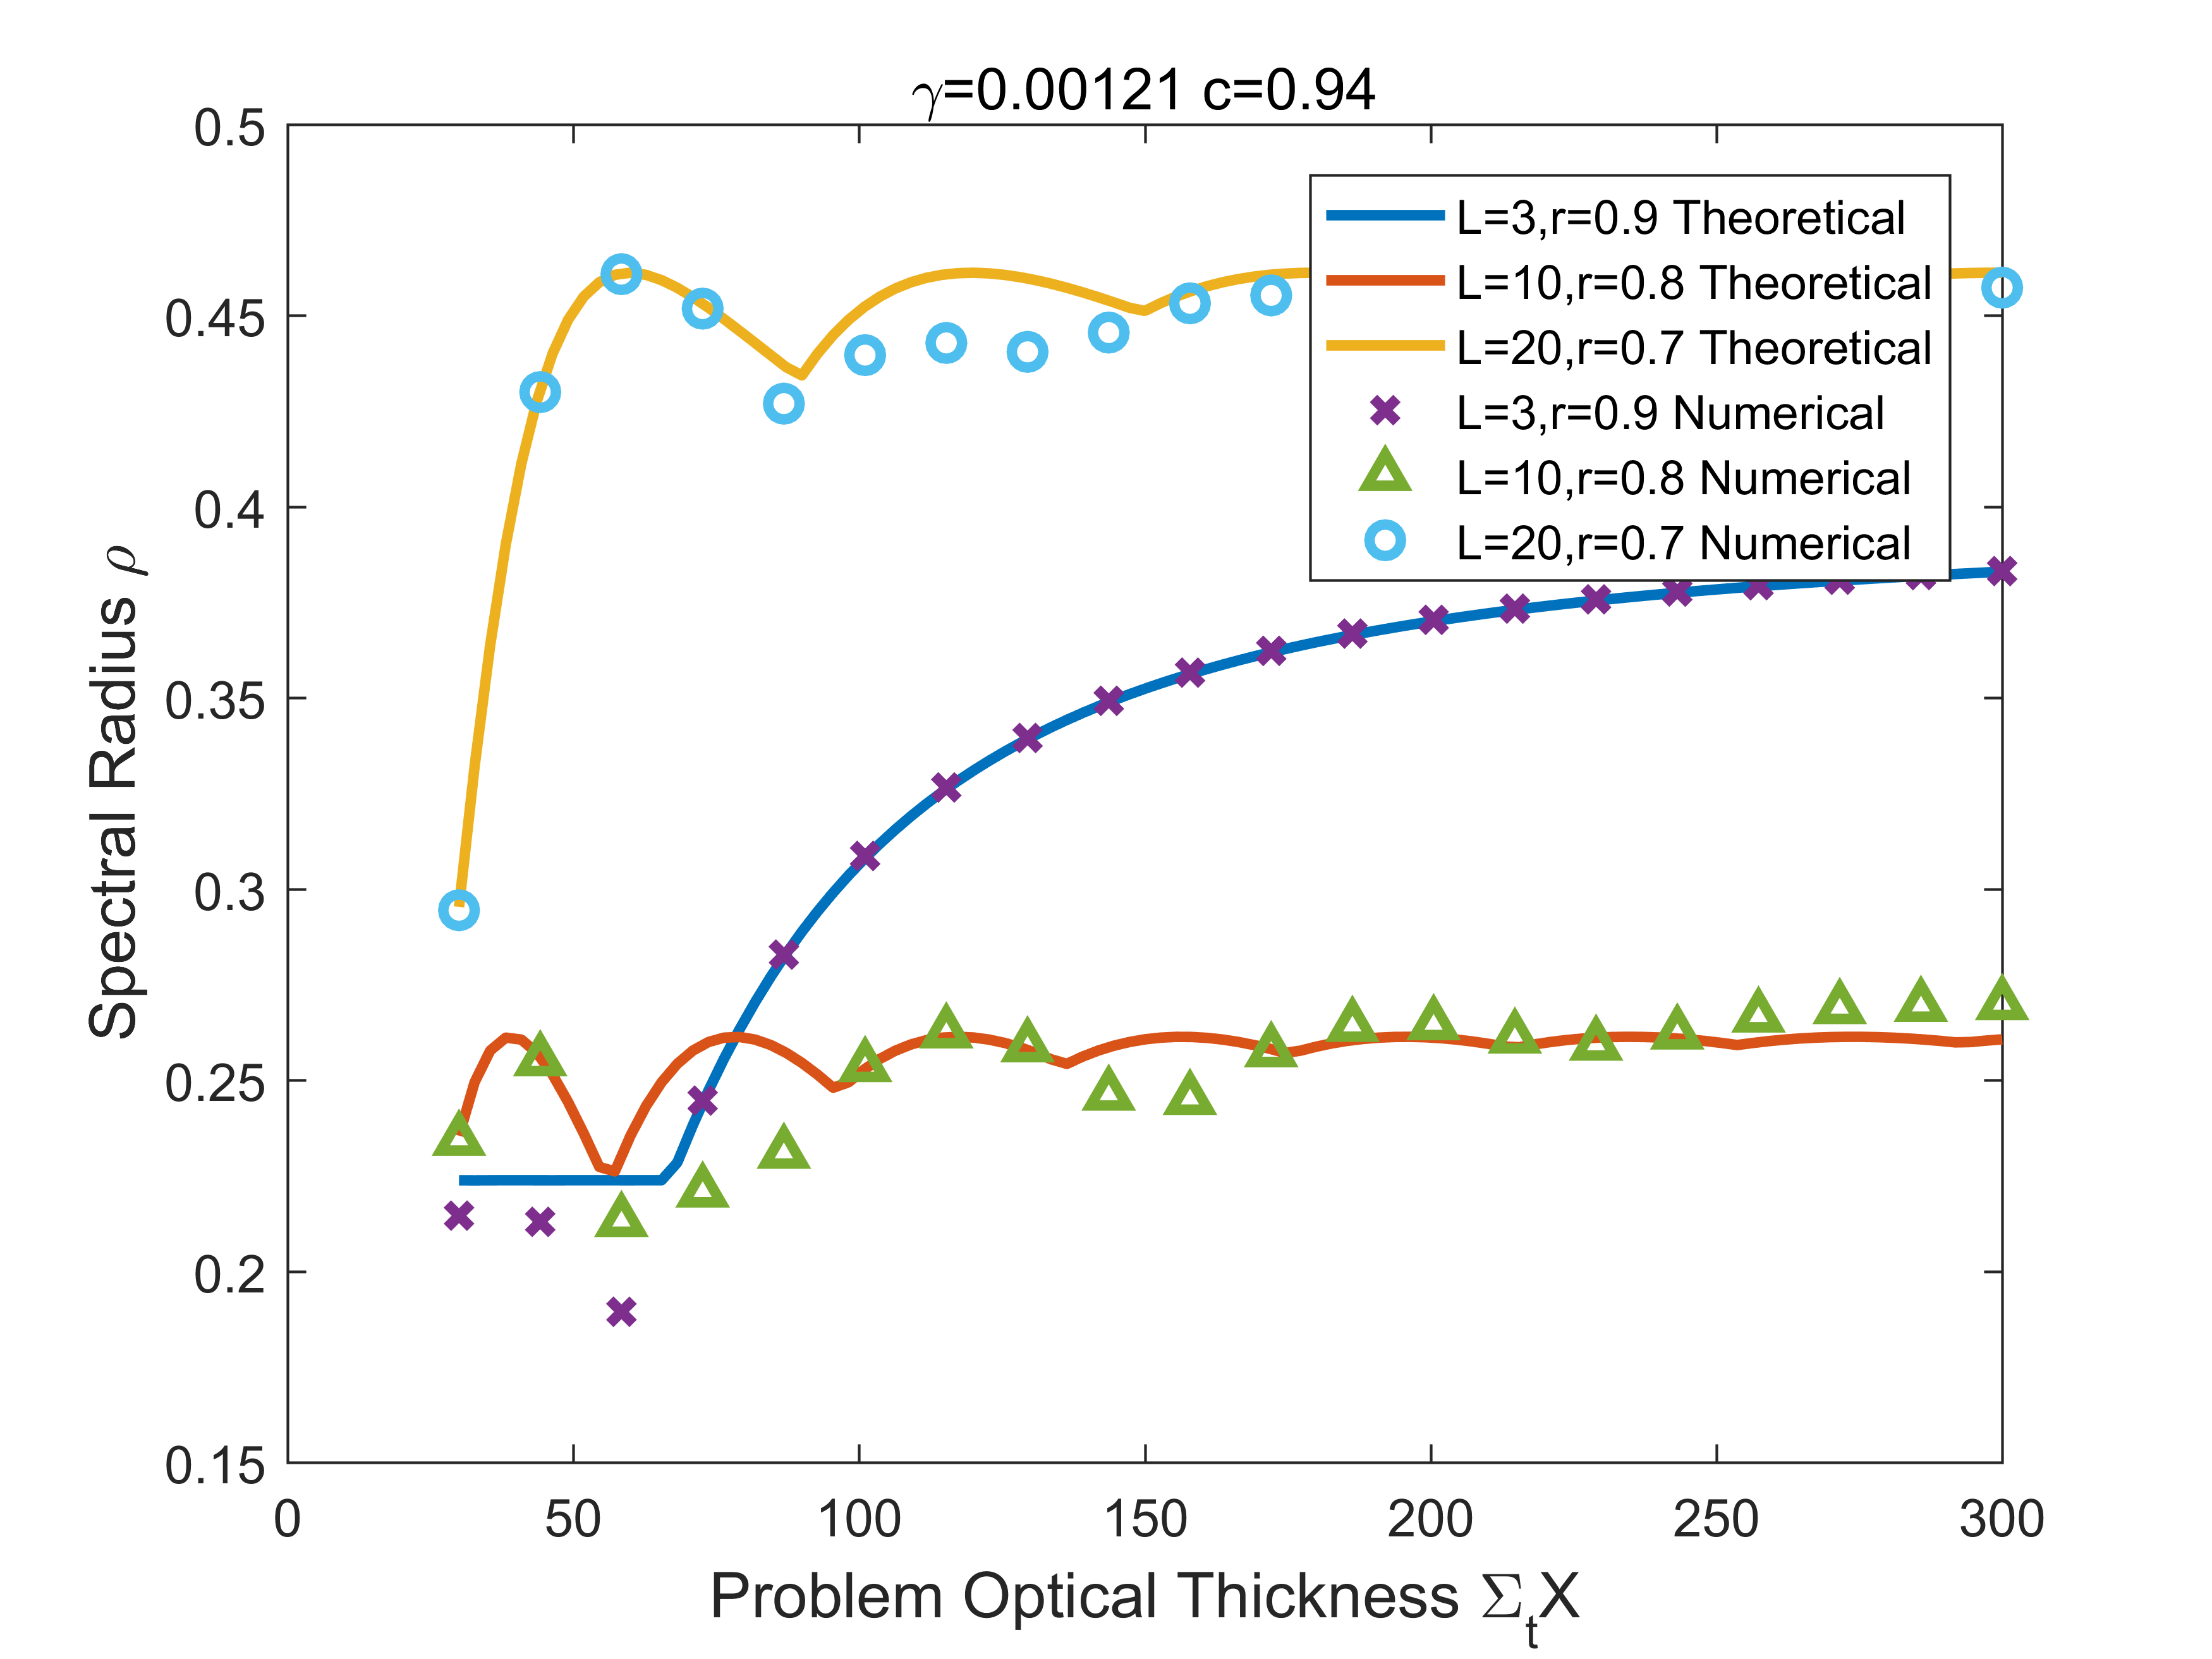
\includegraphics[width=\textwidth]{Texfile/Figure/TheovN_CT.png}
	\end{subfigure}
	\begin{subfigure}[t]{0.4\textwidth}
		\centering
		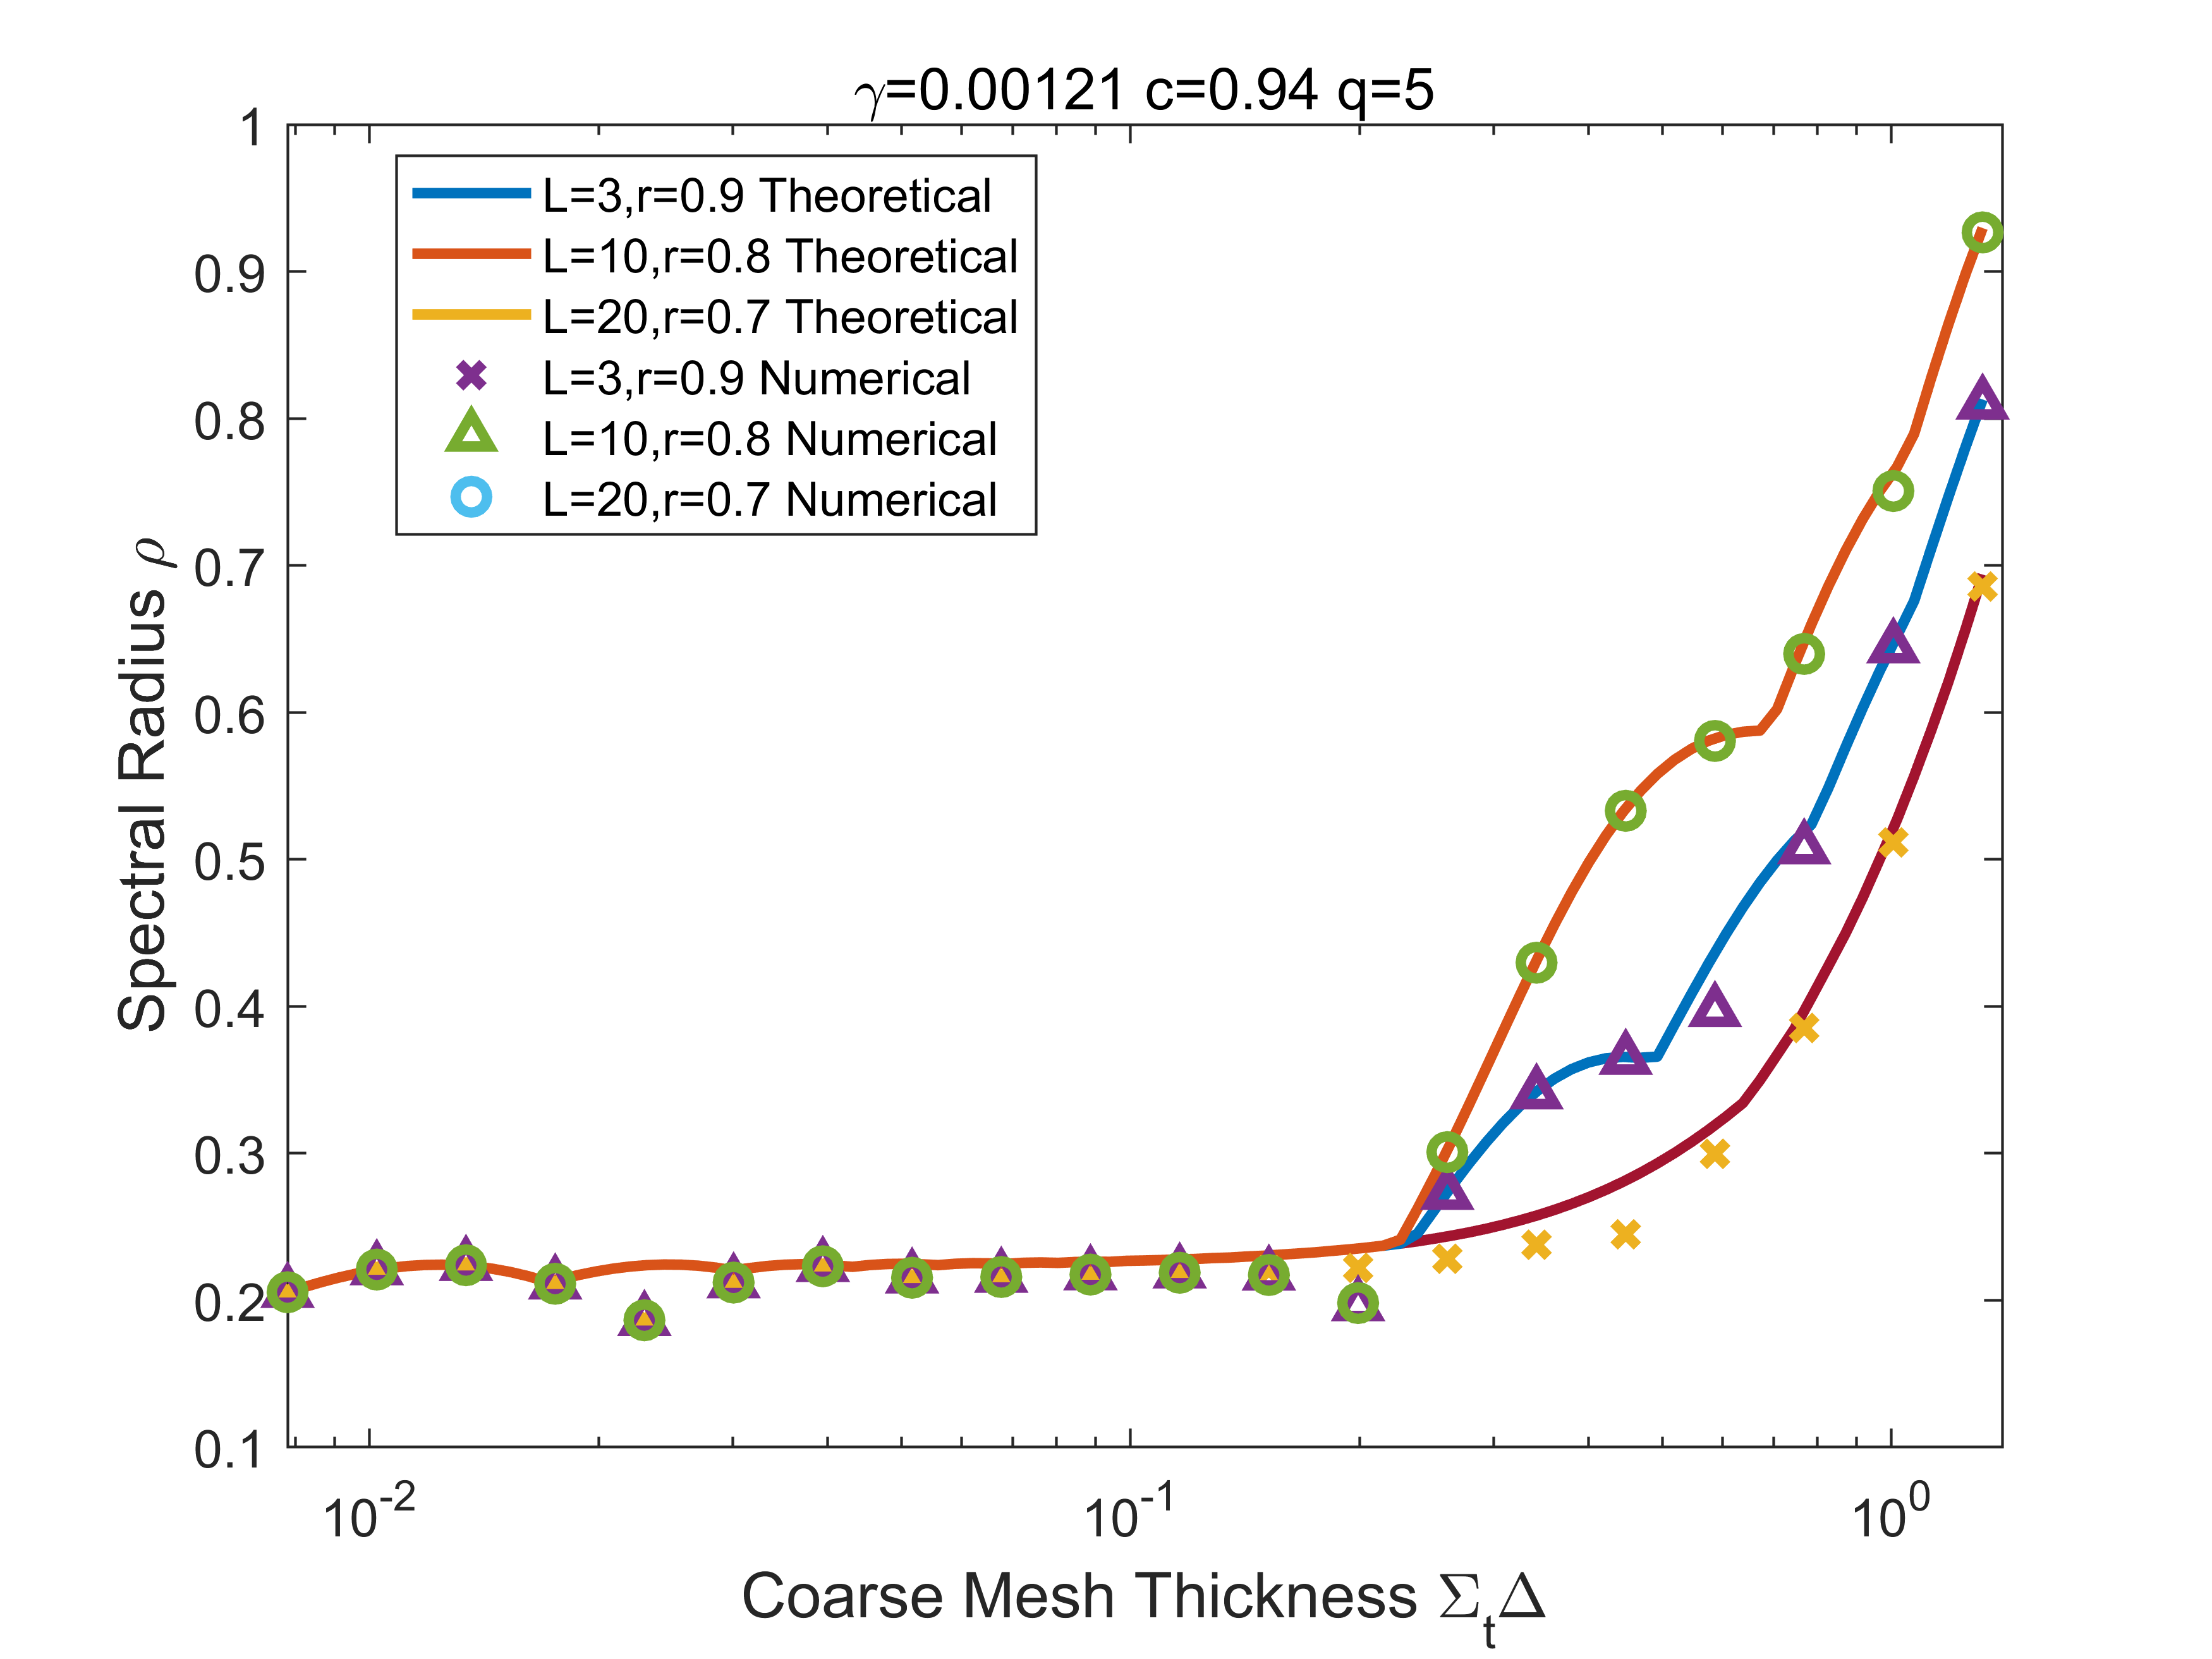
\includegraphics[width=\textwidth]{Texfile/Figure//TheovN_DT.png}
	\end{subfigure}
\end{figure} 

\vspace{-1.5em}
\begin{itemize}
    \item $L$,$r$ are randomly selected to make validation convincing. 
    \vspace{-0.5em}
    \item Wave shape of spectral radius indicates that the effect of partial convergence are problem dependent.
    \vspace{-0.5em}
    \item Fourier analysis predictions agree well with the numerical results from a test code.
\end{itemize}   
\end{frame}


%%%%%%%%%%%%%%%%%%%%%%%%%%%%%%%%%%%%%%%%%%%%%%%%%%%%
\begin{frame}{Effect of Power Iteration Number}
\vspace{-1em}
 \begin{figure}
	\centering
	\captionsetup[subfigure]{justification=centering}
	\begin{subfigure}[t]{0.4\textwidth}
		\centering
 		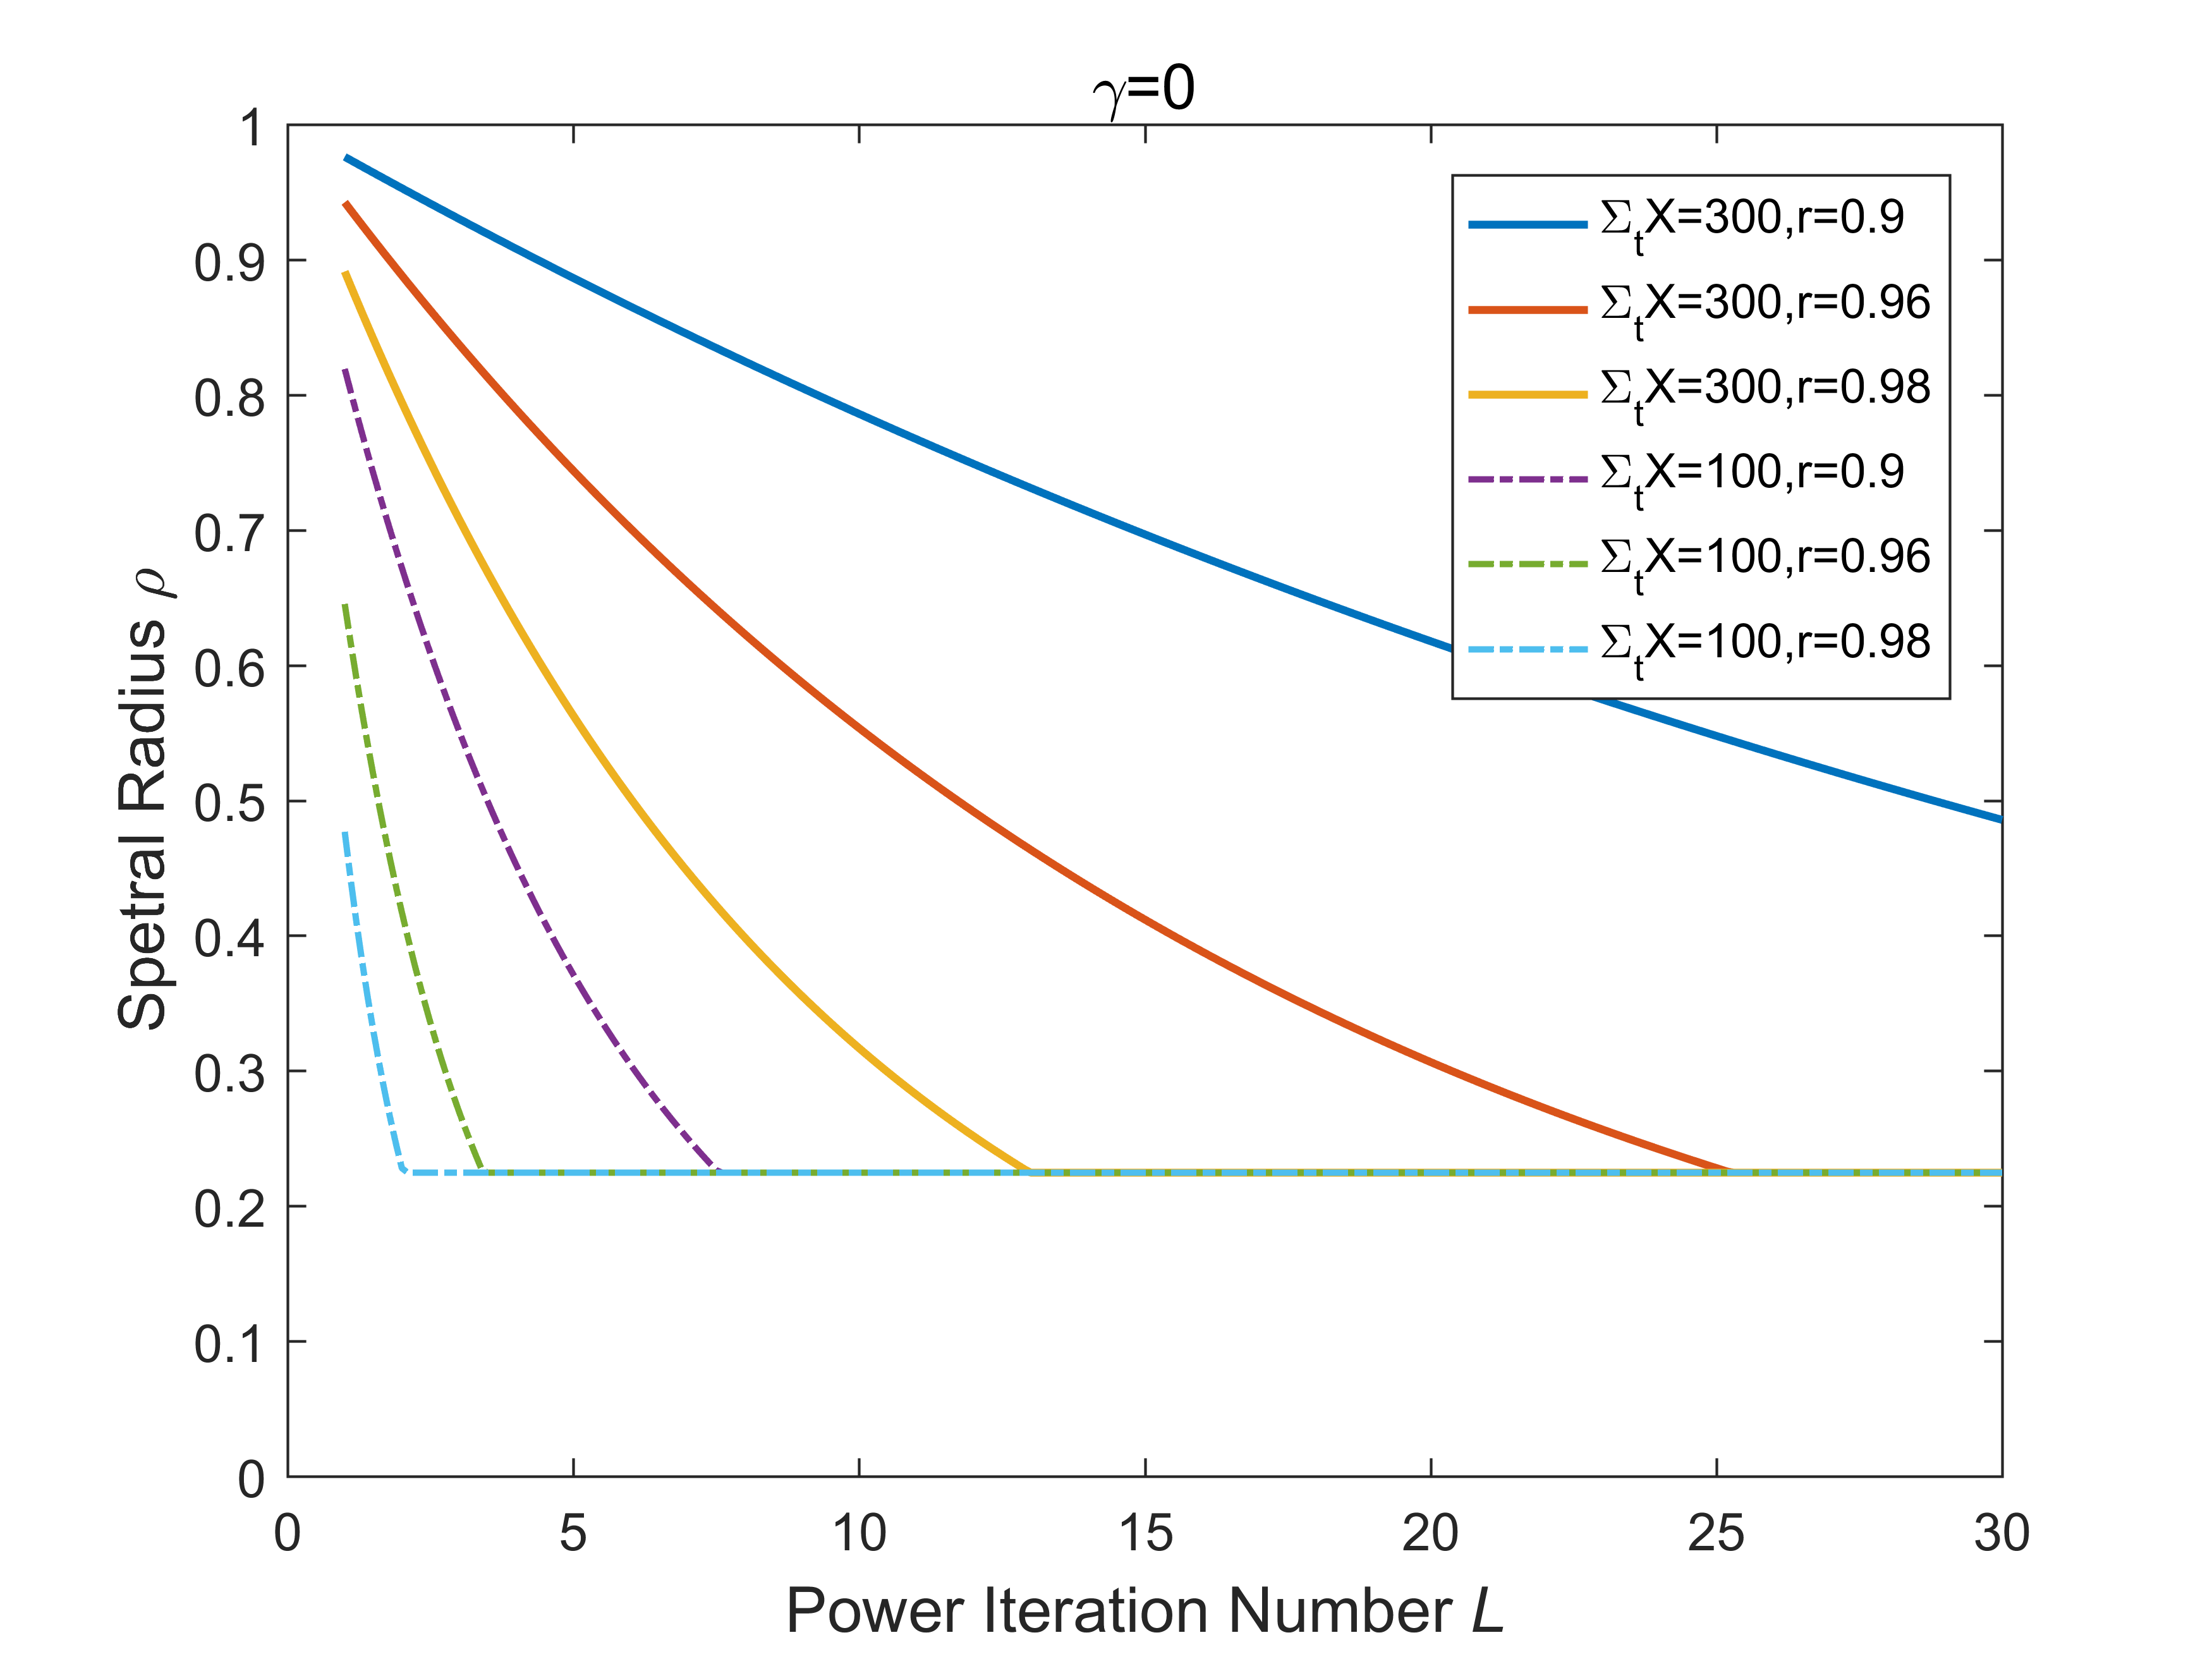
\includegraphics[width=\textwidth]{Texfile/Figure/noFeedback.png}
	\end{subfigure}
	\begin{subfigure}[t]{0.4\textwidth}
		\centering
		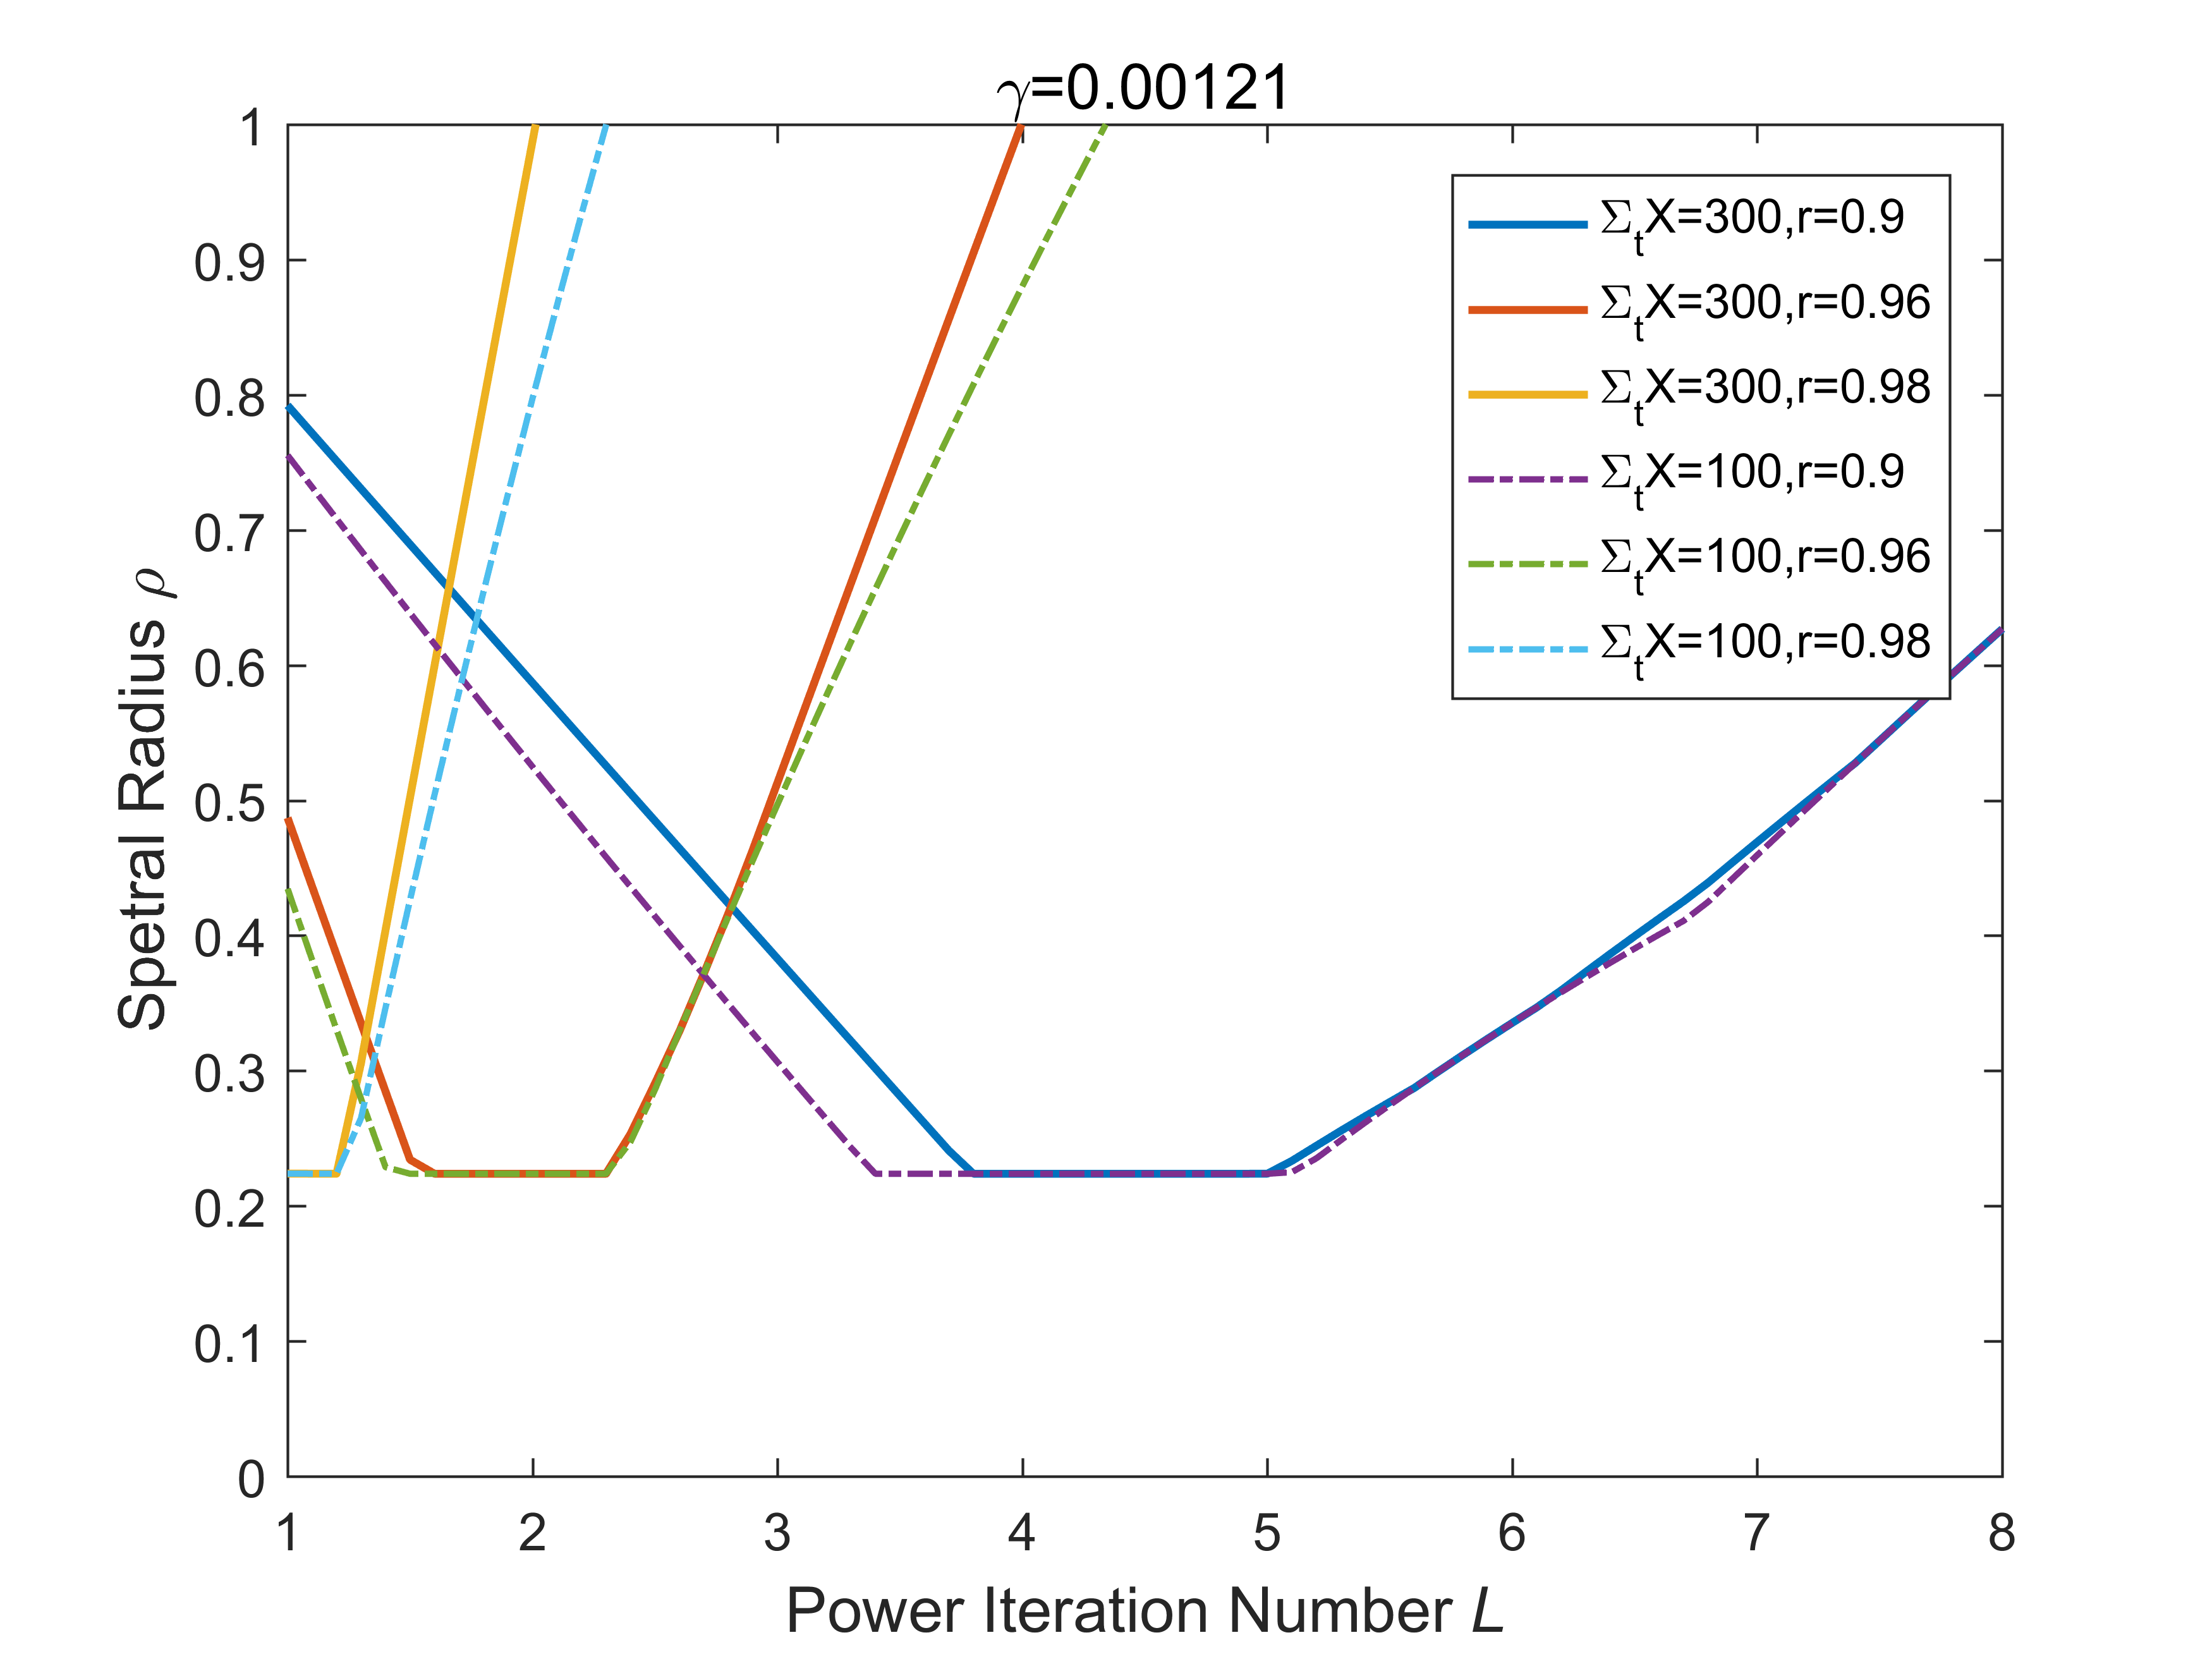
\includegraphics[width=\textwidth]{Texfile/Figure/Feedback_n.png}
	\end{subfigure}
\end{figure} 
\vspace{-1.5em}
\begin{itemize}
    \item Tightening the convergence of NDA by increasing the power iteration number or aggressiveness of Wielandt Shift will stablize the problem without feedback.
    \vspace{-0.7em}
    \item However, it will make the Picard scheme become more stable first, then more unstable till unconverged (similiar with the relaxation).
    \vspace{-0.7em}
    \item Near-optimal partial convergence exists but is problem-dependent.
\end{itemize}   
\end{frame}
% \begin{frame}{Effect of Power Iteration Number (Cont'd)}
% \vspace{-1em}
%  \begin{figure}
% 	\centering
% 	\captionsetup[subfigure]{justification=centering}
% 	\begin{subfigure}[t]{0.4\textwidth}
% 		\centering
%  		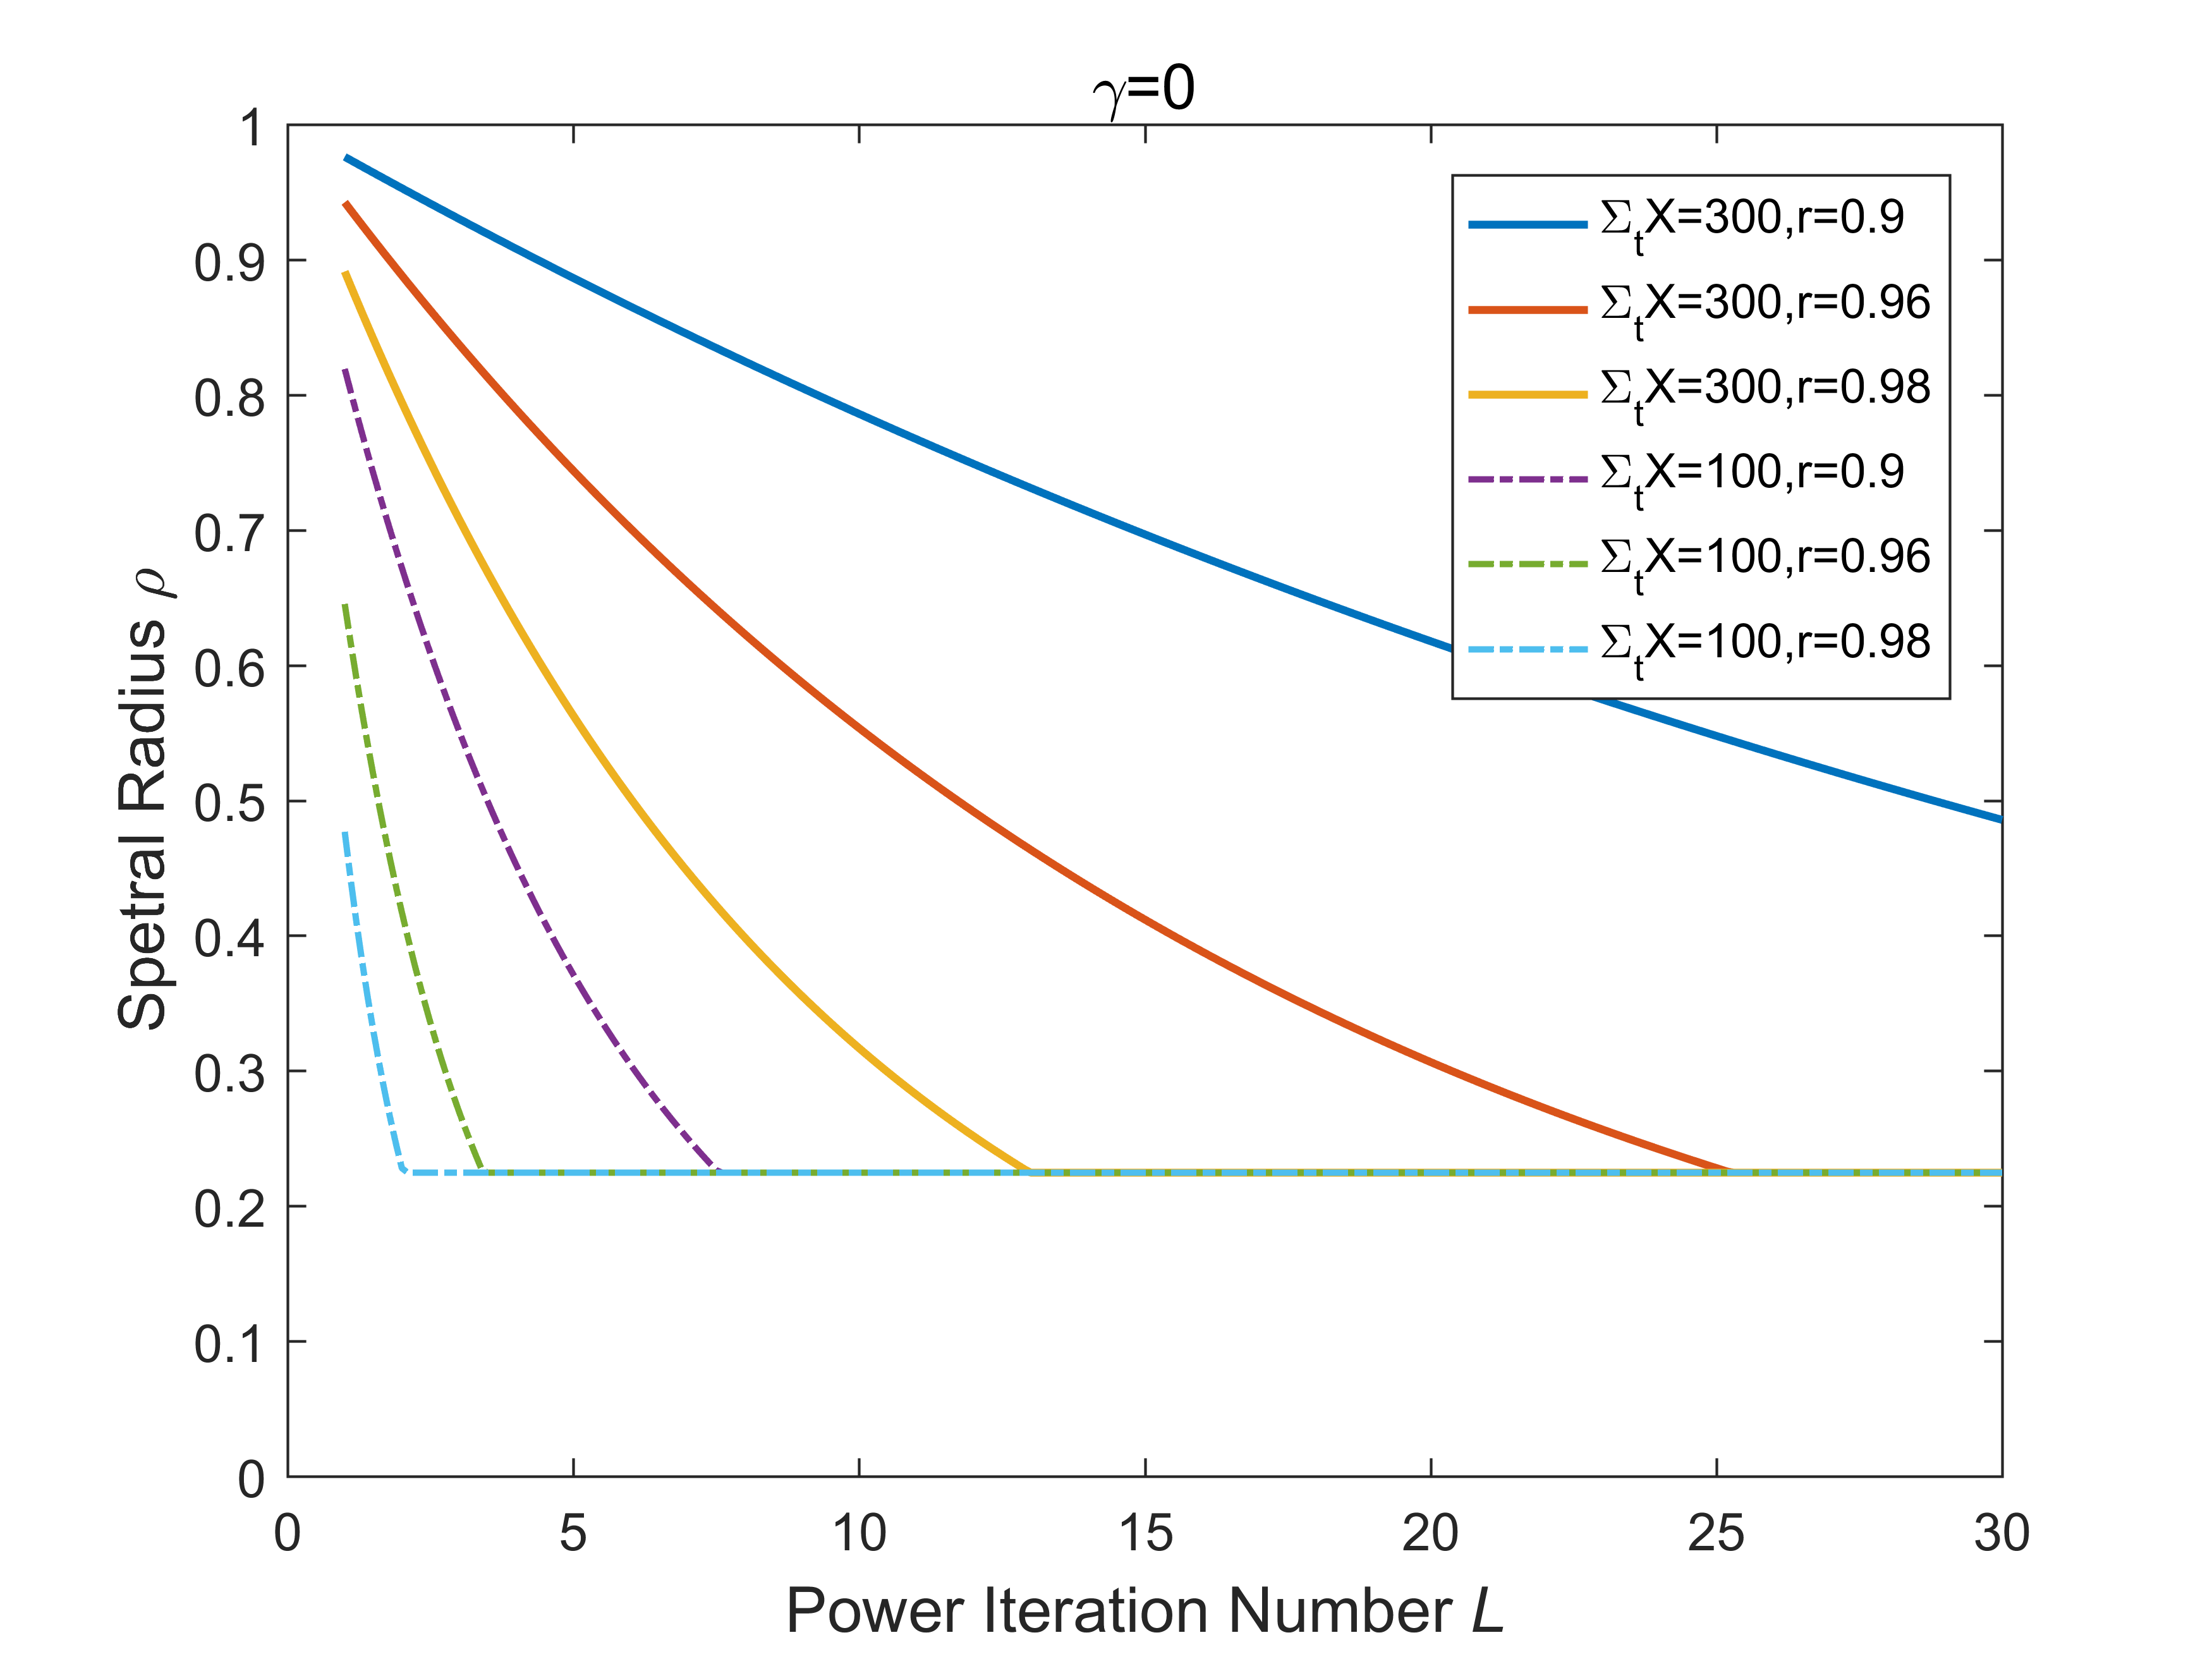
\includegraphics[width=\textwidth]{Texfile/Figure/noFeedback.png}
% 	\end{subfigure}
% 	\begin{subfigure}[t]{0.4\textwidth}
% 		\centering
% 		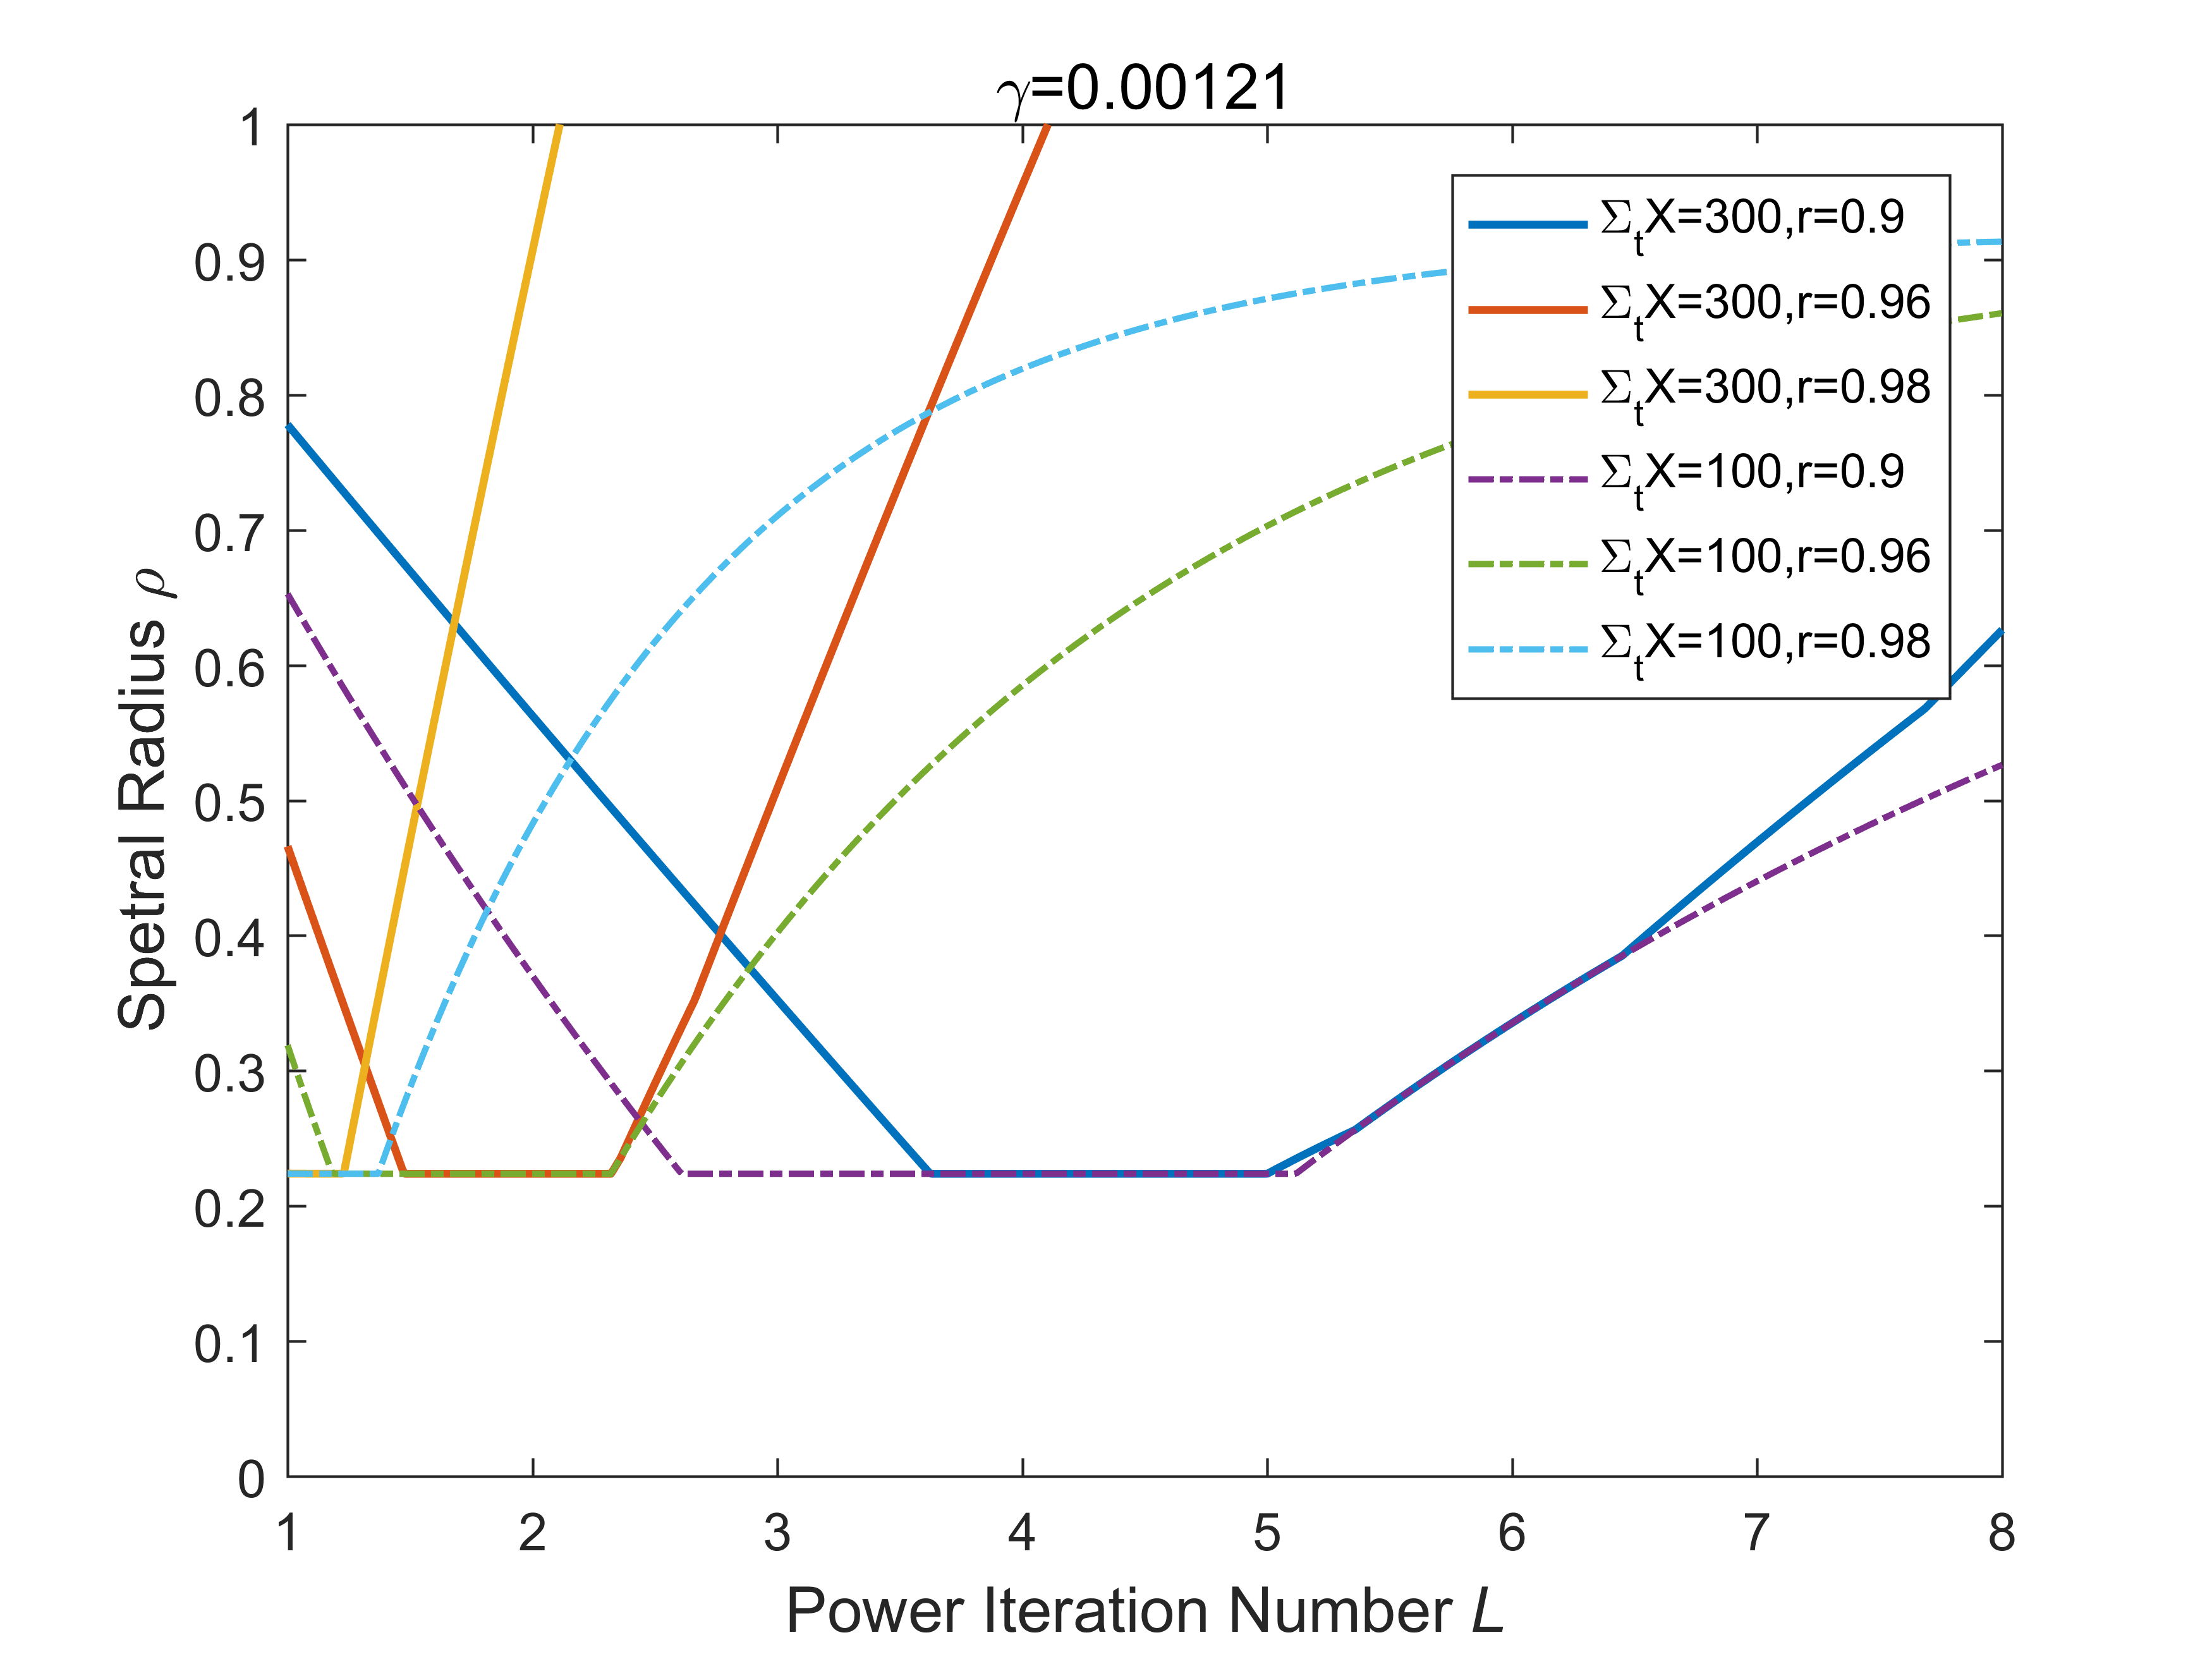
\includegraphics[width=\textwidth]{Texfile/Figure/Feedback.png}
% 	\end{subfigure}
% \end{figure} 
% \vspace{-1.5em}
% \begin{itemize}
%     \item \textbf{0.2247} can be achieved with partial convergence for problem with $\Sigma_tX=300$.
%     \vspace{-0.7em}
%     \item \textbf{Takeaway}: Try to fully converge in non-feedback problem. 
%     \item \textbf{Takeaway}: Try not to fully converge the NDA (CMFD) in feedback problem.
% \end{itemize}   
% \end{frame}
%%%%%%%%%%%%%%%%%%%%%%%%%%%%%%%%%%%%%%%%%%%%%%%%%%%%%%%%%%%%%%%%%%%%%%%%%%%%%%%%%%%%%%%%%%%%%%%%%%%%%%%%%%%%%%%%%%%%%%%%%%%%%%%%
\subsection{Relationship between Partial Convergence and Relaxation}
%%%%%%%%%%%%%%%%%%%%%%%%%%%%%%%%%%%%%%%%%%%%%%%%%%%%
\begin{frame}{Fourier Analysis Result of Fully Converged Nonlinear Diffusion Acceleration with Flux Relaxation}

\begin{itemize}
    \item Flux relaxation is applied when using coarse mesh flux to update the transport solution by:
    \begin{equation}
        \phi(x)=\beta\phi_j+(1-\beta)\phi(x)
    \end{equation}
    \item Final Expression:
    \begin{align}\label{eqns:four-theta}
     \theta(\omega)=
        \begin{cases}
        \bSr{1-\beta-\gamma}f_{TS}(\omega)
        +\beta\bBr{f_{NDA}(\omega)-\frac{3\gamma}{\omega^2}f_{TS}(\omega)} \;, &\text{continuous problem}\\
            \max \blr{eig\bSr{\mathbf{T}(\omega)}}\;, \text{discretized problem}
        \end{cases}
\end{align}

    where:
    \begin{align}
    \mathbf{T}(\omega)=\tilde{\mathbf{H}}(\omega)(1-\gamma)-\beta\mathbf{1}\frac{3\Sigma_t\Delta(e^{i\Sigma_t\Delta\omega}-1)\tilde{\mathbf{G}}+\gamma3(\Sigma_t\Delta)^2\frac{\mathbf{1}^T}{q}\tilde{\mathbf{H}}}{2-2cos(\Sigma_t\Delta\omega)} \label{eq:eror_tr_mtx}
    \end{align} 
\end{itemize}  
\end{frame}

%%%%%%%%%%%%%%%%%%%%%%%%%%%%%%%%%%%%%%%%%%%%%%%%%%%%%%%%%%%%%%%%%%%%%%%%%%%%%%%%%%%%%%%%%%%%%%%%%%%%%%%%%%%%%%%%%%%%%%%%%%%%%%%%
\begin{frame}{Relation between Partial Convergence and Flux Relaxation}
\vspace{-1em}
 \begin{figure}
	\centering
	\captionsetup[subfigure]{justification=centering}
	\begin{subfigure}[t]{0.45\textwidth}
		\centering
 		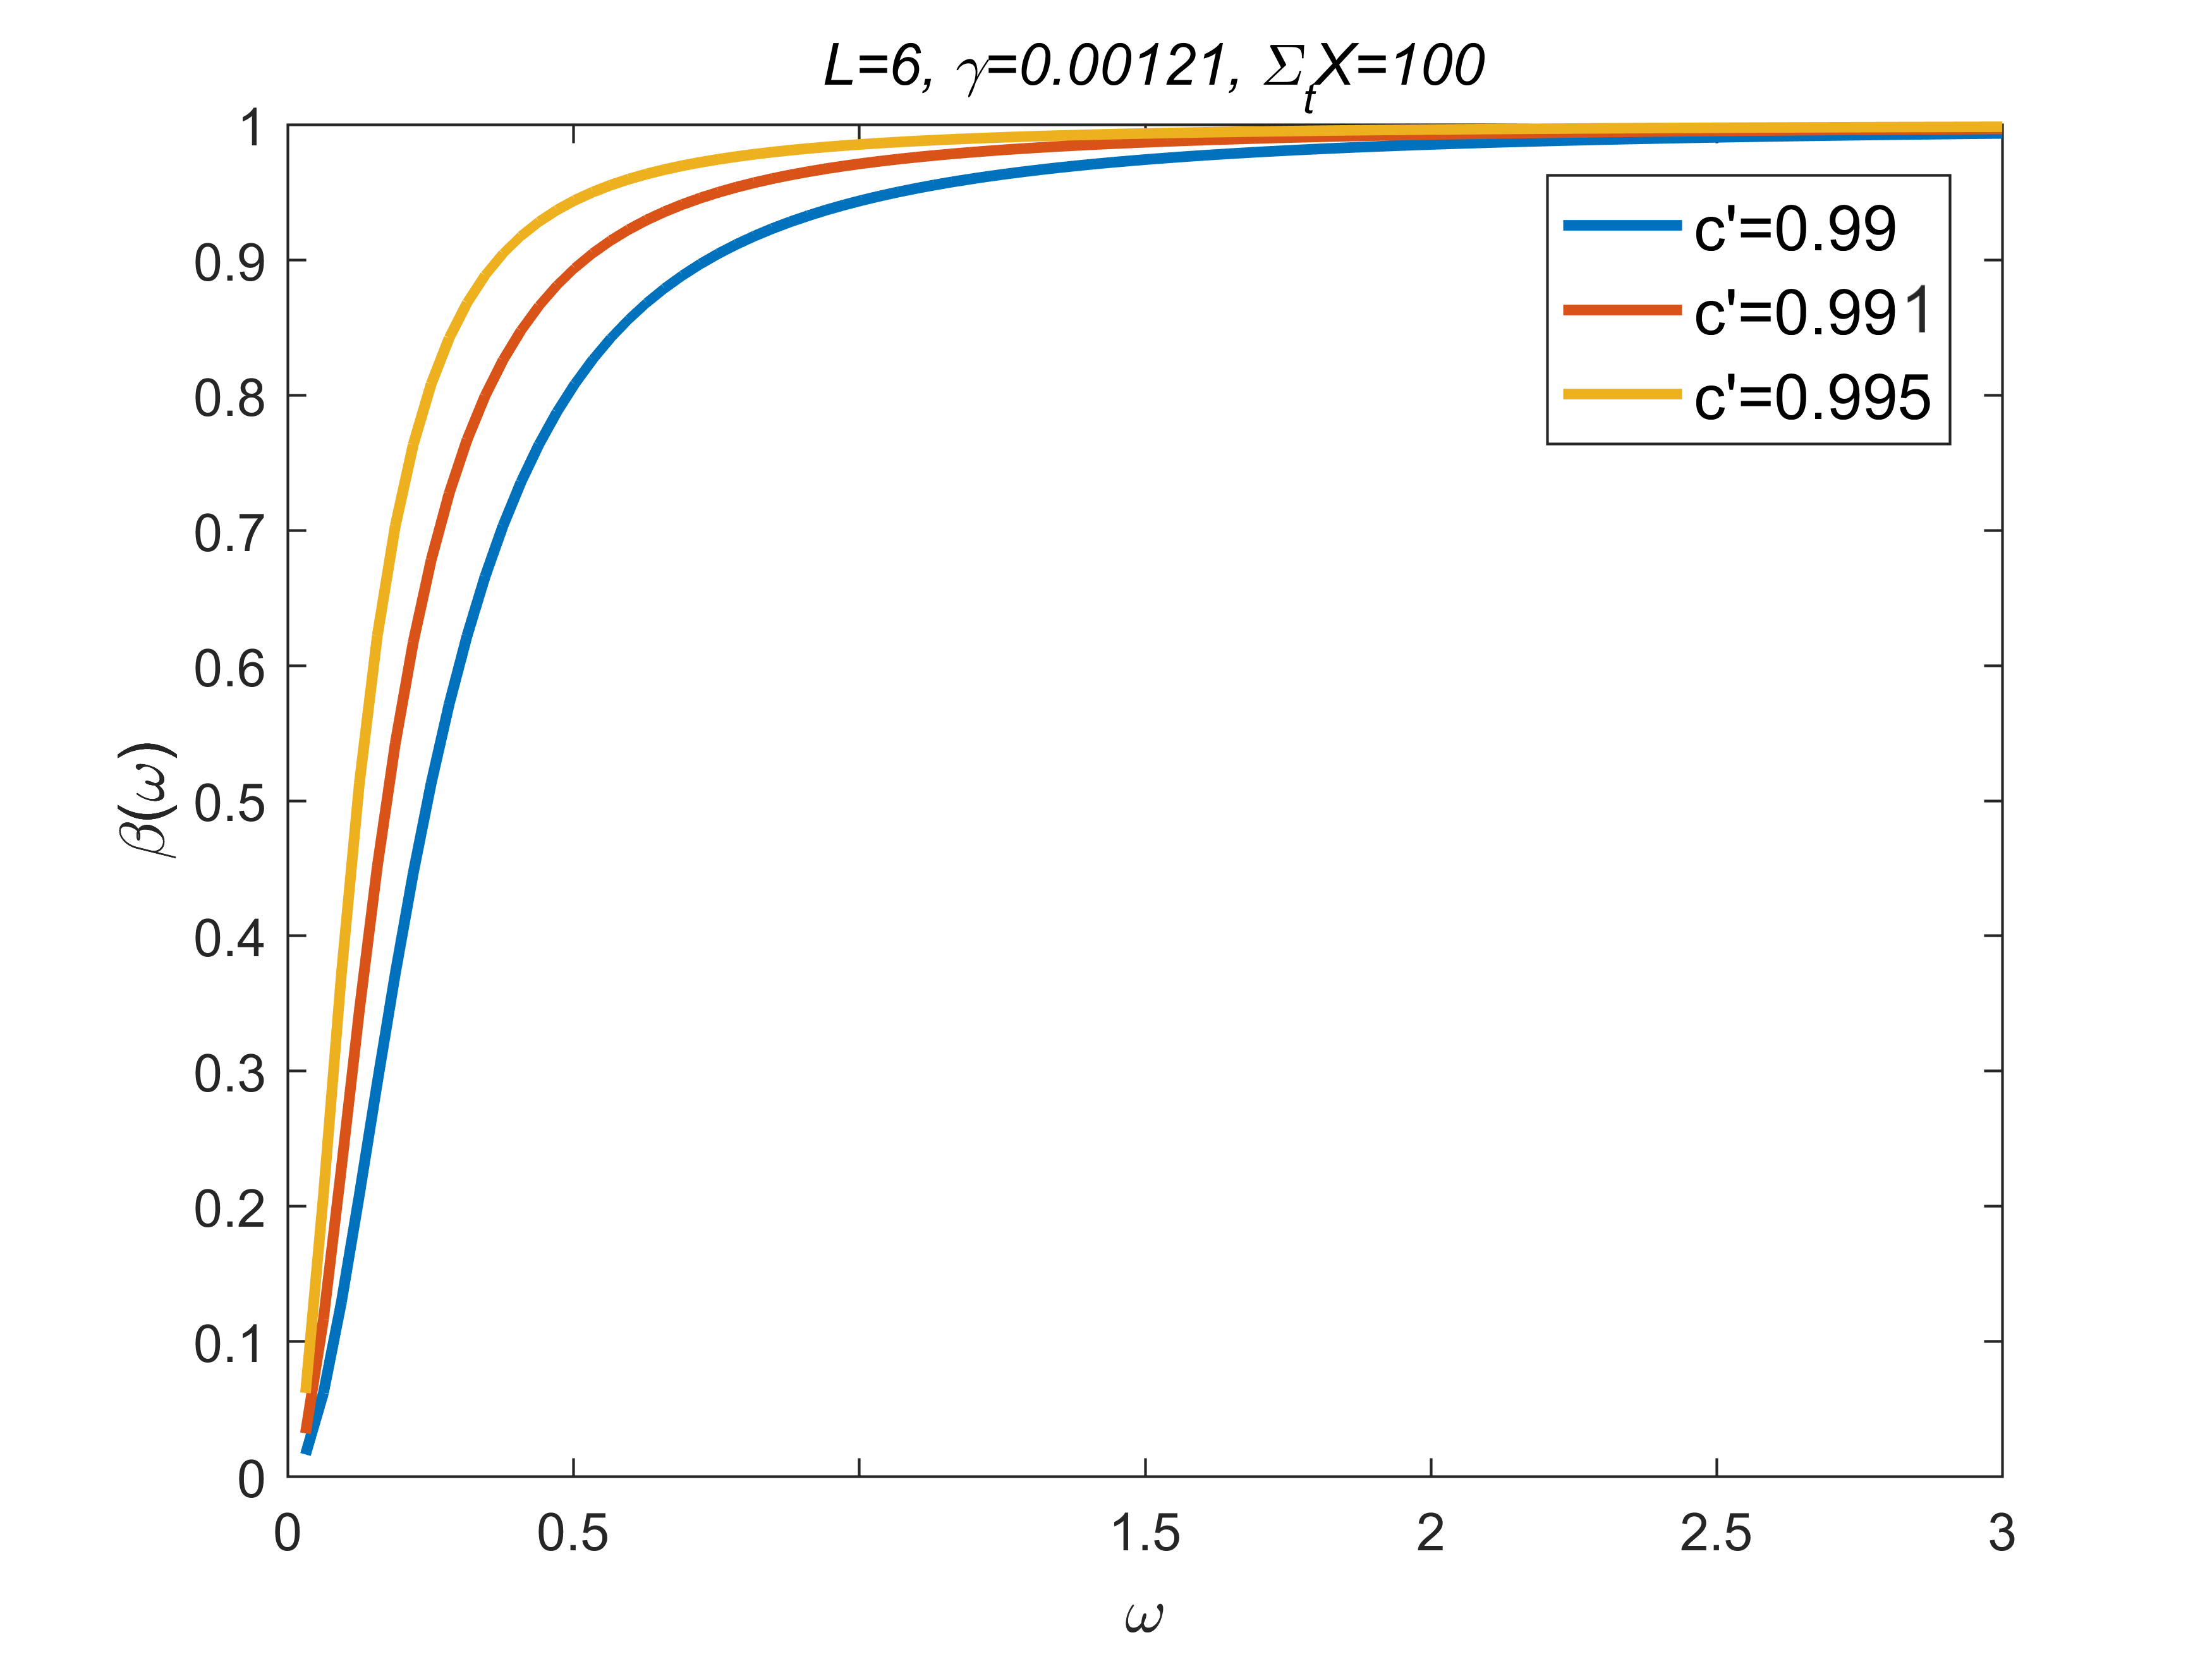
\includegraphics[width=\textwidth]{Texfile/Figure/betavomega.png}
	\end{subfigure}
	\begin{subfigure}[t]{0.45\textwidth}
		\centering
		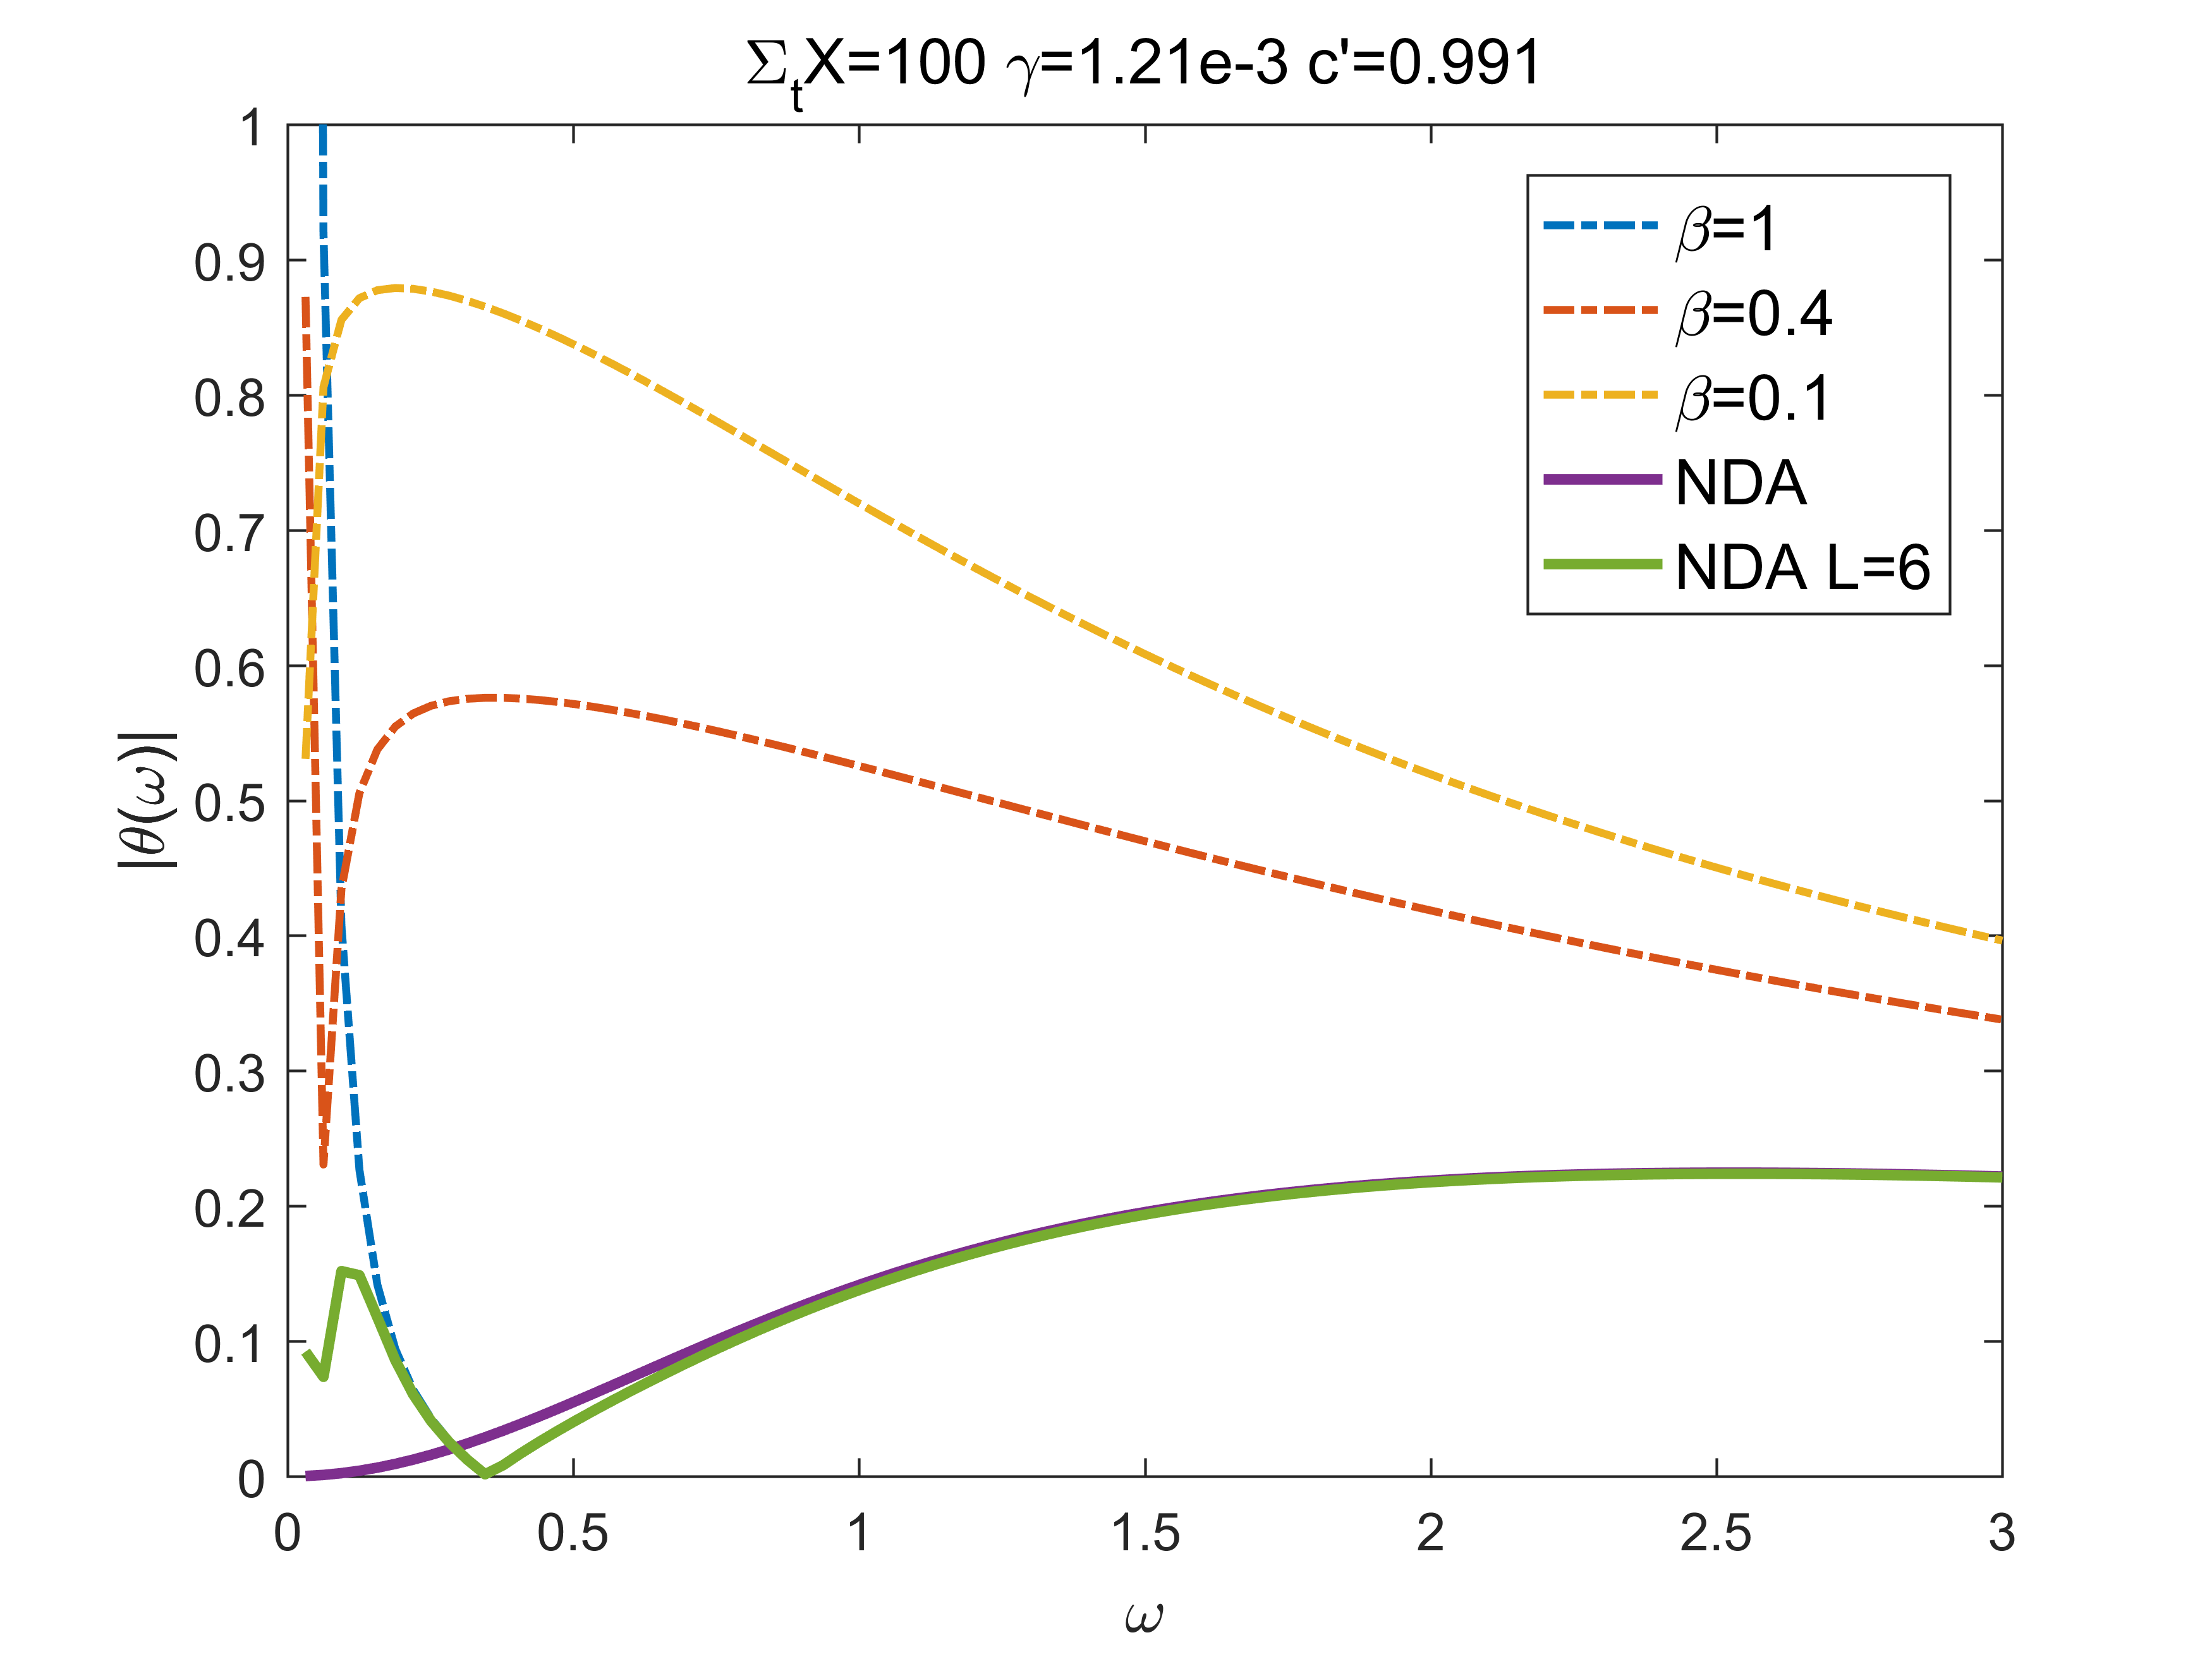
\includegraphics[width=\textwidth]{Texfile/Figure/rhovo_n.png}
	\end{subfigure}
\end{figure} 
\vspace{-1.5em}
\begin{itemize}
    \item Partial convergence induces the Fourier-frequency-dependent flux relaxation factor:
    \vspace{-0.5em}
    \begin{equation}\label{eq:betad}
        \beta(\omega)=1-\Lambda^L(\omega).
    \end{equation}\\
    \vspace{-1.2em}
    \item The relaxation is mainly imposed on the relatively flat Fourier error modes.
\end{itemize}
\end{frame}
%%%%%%%%%%%%%%%%%%%%%%%%%%%%%%%%%%%%%%%%%%%%%%%%%%%%%%%%%%%%%%%%%%%%%%%%%%%%%%%%%%%%%%%%%%%%%%%%%%%%%%%%%%%%%%%%%%%%%%%%%%%%%
\subsection{Near-Optimal Partial Convergence}
\begin{frame}{Derivation of the Near-Optimal Partial Convergence}
\vspace{-1em}
 \begin{itemize}
    \item Rewrite the expression for spectral radius as for continuous case:
    \begin{equation}
       \theta(\omega)=\bSr{1-\beta(\omega)-\gamma-\beta(\omega)\frac{3\gamma}{\omega^2}}f_{TS}(\omega)
        +\beta(\omega)f_{NDA} 
    \end{equation}
    \item For relatively flat fourier modes, $f_{TS}(\omega)\approx 1$
    \item The near optimal partial convergence should make:
    \vspace{-0.2cm}
    \begin{equation}
        1-\beta(\omega)-\gamma-\beta(\omega)\frac{3\gamma}{\omega^2}\approx0
    \end{equation}
    \vspace{-1em}
    the near-optimal partial convergence in term of wielandt shift is:
    \begin{equation}\label{eq:opr}
        r=1-\frac{\left(1-\beta(\omega)\right)^{\frac{1}{L}}}{1-\left(1-\beta(\omega)\right)^{\frac{1}{L}}}\frac{\omega^2}{3(1-c)}.
    \end{equation}   
     \vspace{-1em}
\end{itemize}  
\end{frame}
%%%%%%%%%%%%%%%%%%%%%%%%%%%%%%%%%%%%%%%%%%%%%%%%%%%%%%%%%%%%%%%%%%%%%%%%%%%%%%%%%%%%%%%%%%%%%%%%%
\begin{frame}{Test of Near-Optimal Partial Convergence}
\vspace{-1em}
 \begin{figure}
	\centering
	\captionsetup[subfigure]{justification=centering}
	\begin{subfigure}[t]{0.45\textwidth}
		\centering
 		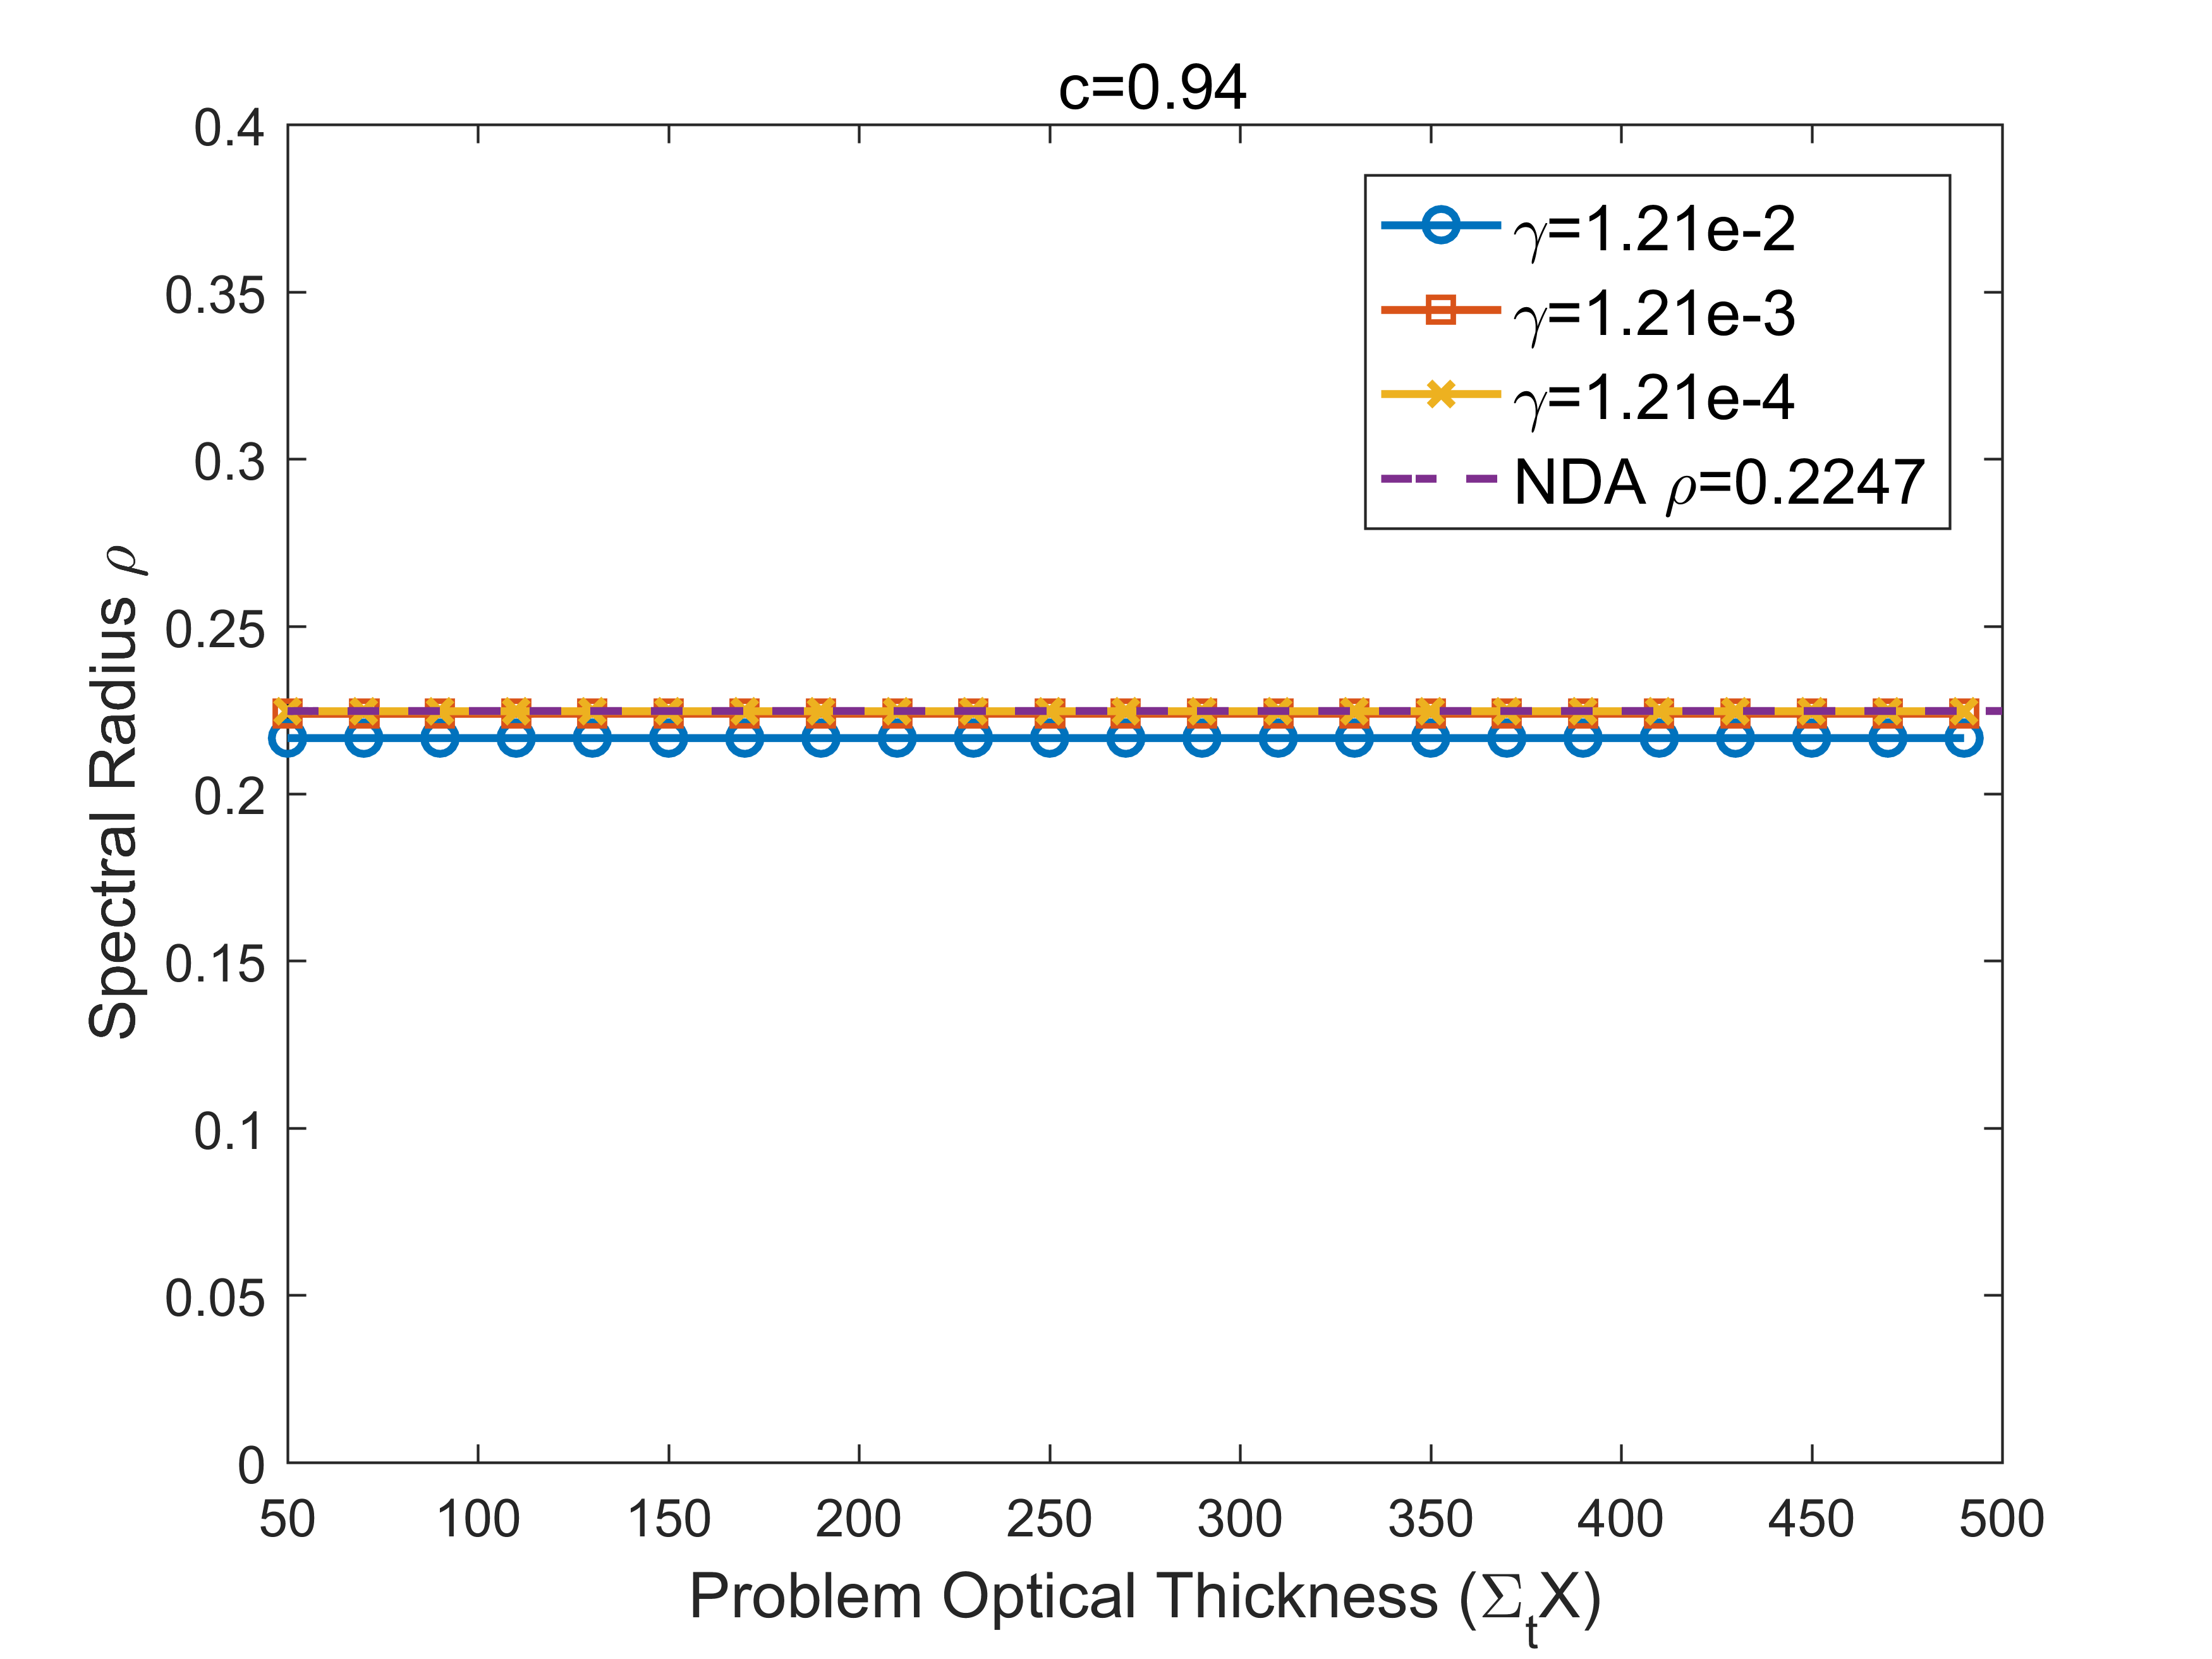
\includegraphics[width=\textwidth]{Texfile/Figure/NDAoptimal.png}
	\end{subfigure}
	\begin{subfigure}[t]{0.45\textwidth}
		\centering
		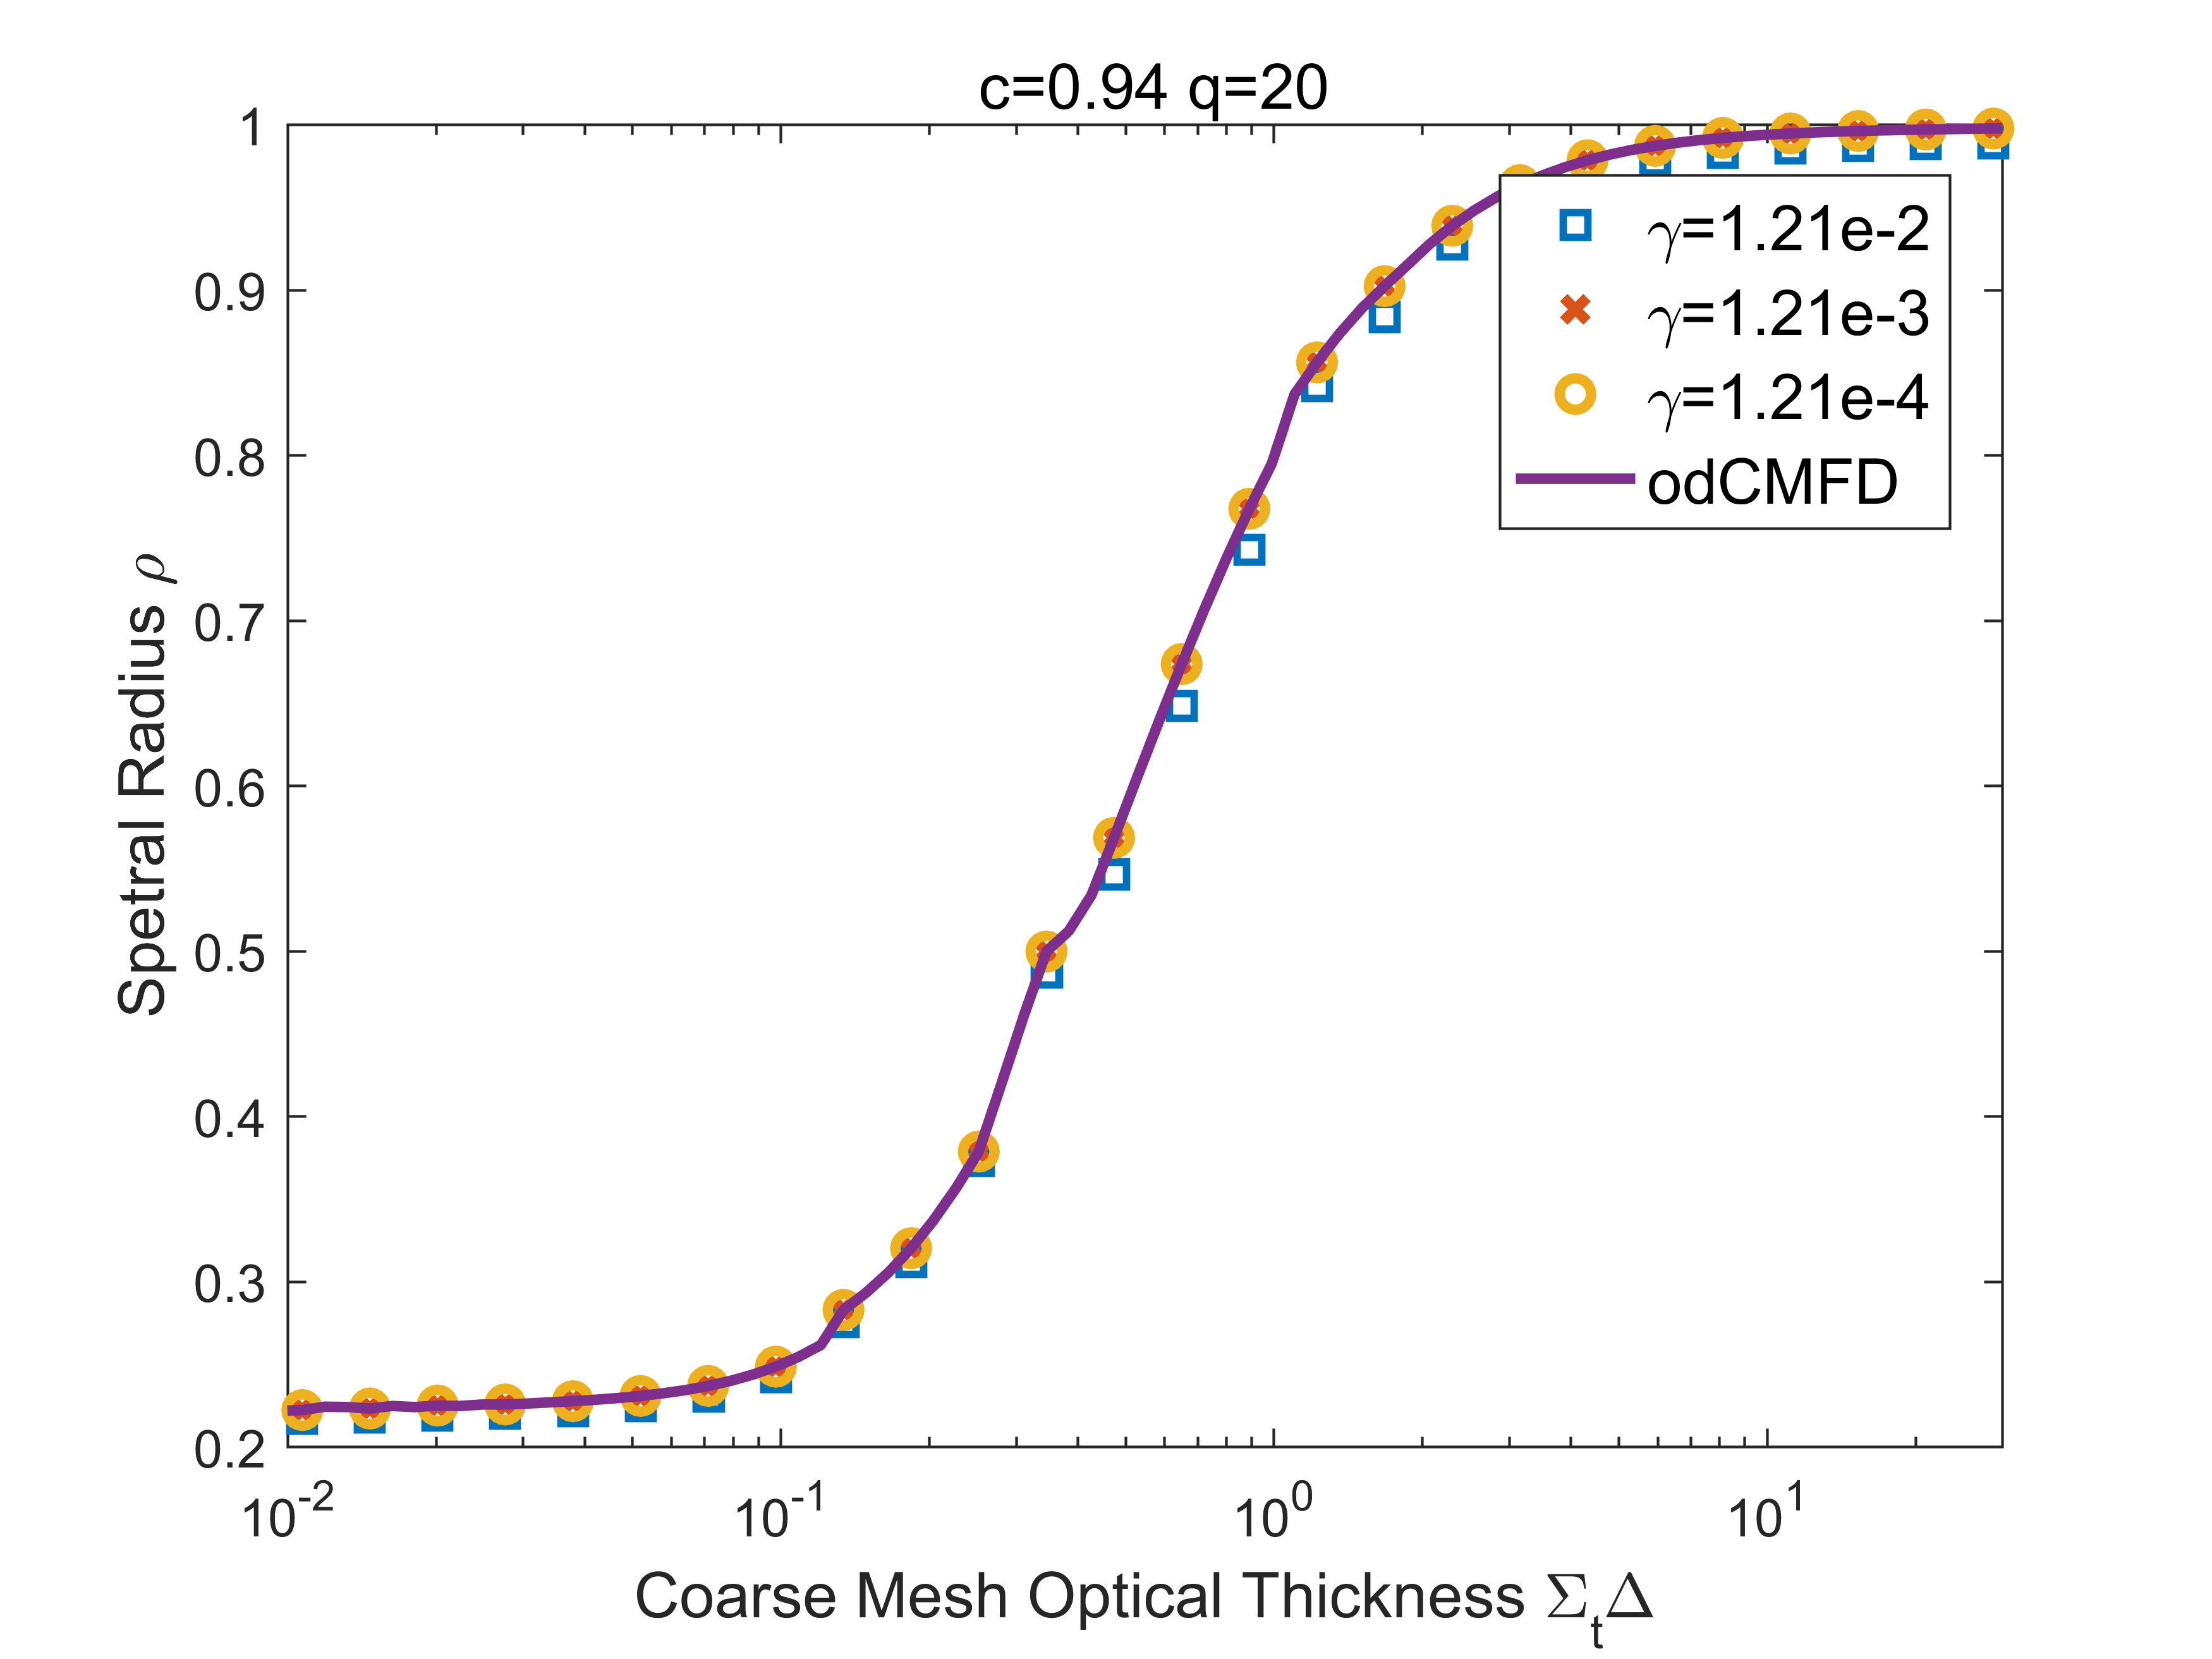
\includegraphics[width=\textwidth]{Texfile/Figure/CMFDoptimal.png}
	\end{subfigure}
\end{figure} 
\vspace{-1.5em}
\begin{itemize}
    \item $\omega=\frac{\pi}{200}$ is suggested.
    \item The same convergence behavior as NDA(CMFD) can be achieved theoretically.
\end{itemize}
\end{frame}
%%%%%%%%%%%%%%%%%%%%%%%%%%%%%%%%%%%%%%%%%%%%%%%%%%%%%%%%%%%%%%%%%%%%%%%%%%%%%%
\begin{frame}{Discussion of Near-optimal Partial Convergence}
\vspace{-1em}
 \begin{itemize}
     \item Pros:
     \begin{itemize}
         \item Easily to be implemented. Compatible with the CMFD and mutlilevel method such as MSED and Multilevel CMFD.
         \item Stablize the scheme and reduce the computational intensity.
     \end{itemize}
     \item Cons:
     \begin{itemize}
         \item $\gamma$ term needed to be calculated
         \item Derivation is based on $NDA$, may not be optimal for CMFD.
     \end{itemize}
     \item Conclusion: Intermediate solution to stabilize the Picard scheme with better efficiency. 
 \end{itemize}
 \end{frame}

